\documentclass[11pt,a4paper]{article}

% ---------- PACKAGES ----------
\usepackage[margin=2.2cm]{geometry}
\usepackage{iftex}
\ifPDFTeX
  \usepackage[utf8]{inputenc}
\fi
\usepackage[T1]{fontenc}
\usepackage{lmodern}
\usepackage{microtype}
\usepackage{titlesec}
\usepackage{enumitem}
\usepackage{booktabs}
\usepackage{longtable}
\usepackage{array}
\usepackage{tabularx}
\usepackage{xcolor}
\usepackage{pifont}
\usepackage{tikz}
\usetikzlibrary{shapes.geometric,arrows.meta,positioning,fit,backgrounds,calc}
\usepackage{pdflscape}
\usepackage{fancyhdr}
\usepackage{caption}
\usepackage{amssymb}
\usepackage{amsmath}
\usepackage{multirow}
\usepackage{ragged2e}
\usepackage{parskip}
\usepackage{setspace}
\usepackage{graphicx}
\usepackage[colorlinks=true,
linkcolor=blue!55!black,
citecolor=blue!55!black,
urlcolor=blue!55!black,
linktoc=all]{hyperref}

% ---------- COLORS ----------
\definecolor{traceblue}{RGB}{22,54,92}
\definecolor{tracelight}{RGB}{235,241,249}
\definecolor{tracegray}{RGB}{90,90,90}
\definecolor{yesgreen}{RGB}{20,110,60}
\definecolor{nored}{RGB}{150,30,30}
\definecolor{partialorange}{RGB}{170,110,10}

% ---------- SECTION STYLE ----------
\titleformat{\section}
{\normalfont\Large\bfseries\color{traceblue}}
{\thesection.}{0.5em}{}

\titleformat{\subsection}
{\normalfont\large\bfseries\color{traceblue}}
{\thesubsection}{0.5em}{}

\titleformat{\subsubsection}
{\normalfont\normalsize\bfseries\color{tracegray}}
{\thesubsubsection}{0.5em}{}

% ---------- HEADER/FOOTER ----------
\pagestyle{fancy}
\fancyhf{}
\renewcommand{\headrulewidth}{0.4pt}
\fancyhead[L]{\small\textcolor{tracegray}{Invention Disclosure Report}}
\fancyhead[R]{\small\textcolor{tracegray}{TRACE v2.0}}
\fancyfoot[C]{\small\thepage}

% ---------- HELPERS ----------
\newcommand{\yes}{\textcolor{yesgreen}{\textbf{Yes}}}
\newcommand{\no}{\textcolor{nored}{No}}
\newcommand{\partialmark}{\textcolor{partialorange}{Partial}}
\newcommand{\tickbox}{\textcolor{yesgreen}{\Large\ding{52}}}
\newcommand{\emptybox}{$\square$}

\newcolumntype{L}[1]{>{\raggedright\arraybackslash}p{#1}}
\newcolumntype{C}[1]{>{\centering\arraybackslash}p{#1}}

\newenvironment{disclaimerbox}
{\begin{center}
 \begin{minipage}{0.95\textwidth}
 \small\itshape\color{tracegray}}
{\end{minipage}
 \end{center}}

\title{\vspace{-1.5cm}}
\date{}

\begin{document}

% ======================================================
% TITLE PAGE
% ======================================================
\begin{titlepage}
\centering
\vspace*{1.5cm}

{\color{traceblue}\rule{0.6\textwidth}{1.2pt}}\\[1.2cm]

{\Huge\bfseries\color{traceblue} TRACE}\\[0.5cm]

{\Large\bfseries Trace-based Runtime Automata for\\
Compliance and Enforcement}\\[1.5cm]

{\large \bfseries
System and Method for Semantic Abstraction, Probabilistic\\
Automata-Based Behavioral Protocol Inference, and Runtime\\
Conformance Verification of Heterogeneous AI-Agent Execution Traces
}\\[2cm]

\begin{tabular}{ll}
\textbf{Version:} & TRACE v2.0 \\
\textbf{Date:} & \today \\
\textbf{Status:} & Implemented research-grade prototype \\
\end{tabular}

\vfill


\vspace{0.7cm}

{\color{traceblue}\rule{0.6\textwidth}{0.8pt}}

\end{titlepage}

\tableofcontents
\thispagestyle{empty}
\newpage

% ======================================================
\section{Title of the Invention}
% ======================================================

\subsection*{Recommended Title}

\begin{center}
\begin{minipage}{0.9\textwidth}
\centering
\large\itshape
``System and Method for Semantic Abstraction, Probabilistic Automata-Based Behavioral
Protocol Inference, and Runtime Conformance Verification of Heterogeneous AI-Agent
Execution Traces''
\end{minipage}
\end{center}

\subsection*{Alternative Titles}

\begin{enumerate}[label=(\alph*)]
\item ``Trace-Based Behavioral Protocol Inference and Hierarchical Runtime Conformance
Checking for Multi-Framework AI Agent Systems''
\item ``Method and System for Inferring Probabilistic Finite-State Behavioral Models from
Heterogeneous Agent Execution Logs and Detecting Runtime Policy Deviations''
\end{enumerate}

The recommended title deliberately identifies the principal technical elements of the
system-level combination: semantic abstraction of heterogeneous traces, probabilistic
automata inference, and runtime conformance verification. The title does not itself
assert that any particular combination satisfies a legal novelty or inventive-step
standard.

% ======================================================
\section{Field / Area of the Invention}
% ======================================================

The invention lies at the intersection of several established technical fields:

\begin{itemize}[leftmargin=1.4em]
\item \textbf{Artificial intelligence / autonomous agent systems} --- systems in which a
large-language-model-driven planner selects and sequences tool invocations, sub-agent
delegations, and memory operations at runtime.

\item \textbf{Software observability and execution-trace analysis} --- capture and
structuring of runtime event streams from distributed, multi-component software systems.

\item \textbf{Automata theory and grammatical inference} --- passive learning of finite-state
and probabilistic finite-state representations from example sequences, including
state-merging approaches such as RPNI, EDSM, and ALERGIA/MDI.

\item \textbf{Runtime verification / software model checking} --- checking an observed
execution against a formal specification, as distinct from exhaustive state-space model
checking of all possible executions.

\item \textbf{Process mining} --- discovery of process models from event logs and
conformance checking of new traces against discovered or specified models.

\item \textbf{Anomaly and intrusion detection} --- behavior-based detection of deviations
from a learned baseline of normal system activity.

\item \textbf{Machine learning} --- semantic representations and clustering techniques
that may be used to normalize action vocabularies across independently developed software
frameworks.

\item \textbf{Cybersecurity / AI safety} --- policy enforcement and safe operation of
autonomous or semi-autonomous software agents that take real-world actions.
\end{itemize}

The present system specifically applies these areas to multi-framework AI-agent execution
traces. Such traces can exhibit stochastic action selection, heterogeneous action
vocabularies, nested delegation, incomplete observations, and behavioral changes over
time.

The implementation evidence described later in this disclosure establishes a working
software prototype and controlled benchmark evaluation. It does not establish production
deployment or universal performance across all agent architectures, hardware, datasets,
or workloads.

% ======================================================
\section{Prior Patents and Publications from Literature}
% ======================================================

The prior-art discussion below is retained from the supplied disclosure and is presented
as a technical comparison rather than a legal patentability opinion. No new prior-art
search is asserted in this revision. The references and publication details are retained
from the supplied material.

\subsection{Patents}

\begin{landscape}
\footnotesize
\begin{longtable}{C{0.7cm} L{3.3cm} C{1.3cm} L{2.5cm} L{4.2cm} L{4.2cm} L{4.2cm}}
\caption{Comparative summary of directly relevant patents.}
\label{tab:patents}\\
\toprule
\textbf{Sl.\ No.} &
\textbf{Patent No.\ / Publication} &
\textbf{Year} &
\textbf{Patent Office / Assignee} &
\textbf{Key Contribution} &
\textbf{Limitation (relative to TRACE)} &
\textbf{Technical Distinction / Proposed Contribution} \\
\midrule
\endfirsthead

\multicolumn{7}{l}{\small\itshape (Table \thetable\ continued)}\\
\toprule
\textbf{Sl.\ No.} &
\textbf{Patent No.\ / Publication} &
\textbf{Year} &
\textbf{Patent Office / Assignee} &
\textbf{Key Contribution} &
\textbf{Limitation (relative to TRACE)} &
\textbf{Technical Distinction / Proposed Contribution} \\
\midrule
\endhead

\bottomrule
\endfoot

\bottomrule
\endlastfoot

1 &
\href{https://patents.google.com/patent/US11989296}
{US~11,989,296~B2} --- ``Program Execution Anomaly Detection for Cybersecurity'' &
2024 (priority 2022) &
USPTO; CybersentryAi, Inc. &
Instruments a supervised program in a model-building mode, trains an acceptable-behavior
model from event sequences, and compares live event sequences against it in an operation
mode; uses preceding event context as model input. &
Operates on a single instrumented program/process; the supplied comparison does not
identify multi-framework symbolic normalization, semantic action abstraction,
probabilistic state-merging inference, bounded delegation modeling, or explicit product
composition with a separately authored policy automaton. &
TRACE combines heterogeneous agent-trace normalization, probabilistic state-merging
inference, bounded hierarchical delegation, and independent learned/policy verification
tracks in one architecture. \\

\addlinespace

2 &
\href{https://patents.google.com/patent/US20180129579A1/en}
{US~2018/0129579~A1} --- ``Systems and Methods with a Realtime Log Analysis Framework''
(LogLens) &
2018 (priority 2016) &
USPTO; NEC Laboratories America, Inc. &
Unsupervised event identification over heterogeneous multi-source logs; constructs
event automata and performs real-time sequence-anomaly detection with dynamic model
updates. &
The described automata are frequency/association-based state machines over log fields,
rather than the TRACE PDFA state-merging representation. The reference does not establish
TRACE's agent-framework normalization, bounded delegation treatment, or separate
policy-automaton product track. &
TRACE uses a probabilistic state-merging representation and adds canonicalization across
agent frameworks, hierarchical delegation handling, and independent explicit-policy
verification. \\

\addlinespace

3 &
\href{https://patents.google.com/patent/EP1063828A3/en}
{EP~1063828~B1 / US~7,369,507~B1} --- ``Method for Identifying the Underlying Finite State
Machines of a Protocol Implementation'' &
2006 (priority 1999) &
EPO / USPTO; Tektronix Inc.\ (later NetScout) &
Learns finite-state representations underlying protocol implementations from example
traces by clustering observed time points into equivalence classes. &
Targets classical communications protocols and does not establish the combination of
stochastic PDFA inference, heterogeneous AI-agent semantic abstraction, bounded
delegation, or separate policy-product verification used by TRACE. &
TRACE applies probabilistic automata inference to AI-agent execution behavior and combines
it with semantic cross-framework normalization, bounded hierarchical composition, and
explicit policy verification. \\

\addlinespace

4 &
\href{https://patents.google.com/patent/US11928629B2/en}
{US~11,928,629~B2} --- ``Graph Encoders for Business Process Anomaly Detection'' &
2023 (filed approximately 2022) &
USPTO; International Business Machines Corporation &
Converts business-process event logs into graph structures, learns graph encodings using
unsupervised ML, and computes process-aware anomaly scores. &
The representation is graph-embedding based rather than an explicit probabilistic
finite-state behavioral model. The supplied reference does not establish TRACE's
hierarchical delegation representation, learned/policy product construction, or
cross-framework agent-trace normalization. &
TRACE retains explicit finite-state transition structure and probabilistic transition
semantics while adding semantic abstraction, bounded delegation, policy composition, and
drift monitoring. \\

\addlinespace

5 &
\href{https://patents.google.com/patent/US9736172}
{US~9,736,172~B2} --- ``Signature-Free Intrusion Detection'' &
2017 (priority 2007) &
USPTO; Avaya Inc.\ (chain of successor assignees) &
Maintains finite-state models for sessions/nodes/protocol combinations and flags
incompatible states or transitions; composes local and global constraints. &
The supplied comparison describes hand-specified finite-state models rather than passive
probabilistic state-merging learning from positive execution traces. It does not establish
semantic cross-framework action abstraction, bounded agent delegation, or drift-driven
model lifecycle management. &
TRACE infers probabilistic behavioral models from execution traces and independently
composes them with an explicit policy DFA, while addressing heterogeneous AI-agent
execution and bounded delegation. \\

\end{longtable}
\end{landscape}

\subsection{Research Publications}

\begin{landscape}
\footnotesize
\begin{longtable}{C{0.7cm} L{3.3cm} C{1.3cm} L{2.5cm} L{4.2cm} L{4.2cm} L{4.2cm}}
\caption{Comparative summary of directly relevant research publications.}
\label{tab:pubs}\\
\toprule
\textbf{Sl.\ No.} &
\textbf{Publication} &
\textbf{Year} &
\textbf{Venue} &
\textbf{Key Contribution} &
\textbf{Limitation (relative to TRACE)} &
\textbf{Technical Distinction / Proposed Contribution} \\
\midrule
\endfirsthead

\multicolumn{7}{l}{\small\itshape (Table \thetable\ continued)}\\
\toprule
\textbf{Sl.\ No.} &
\textbf{Publication} &
\textbf{Year} &
\textbf{Venue} &
\textbf{Key Contribution} &
\textbf{Limitation (relative to TRACE)} &
\textbf{Technical Distinction / Proposed Contribution} \\
\midrule
\endhead

\bottomrule
\endfoot

\bottomrule
\endlastfoot

1 &
J.\ Oncina and P.\ Garc'{i}a, ``Inferring Regular Languages in Polynomial Updated
Time'' &
1992 &
Pattern Recognition and Image Analysis, World Scientific &
Introduces RPNI, a foundational state-merging approach for learning canonical DFAs from
example strings. &
Targets regular-language learning and does not provide probabilistic semantics,
cross-framework AI-agent normalization, hierarchical delegation, or policy-product
verification. &
TRACE does not claim RPNI as inventive. The candidate contribution lies in the surrounding
system that normalizes agent traces, learns probabilistic behavioral models, represents
bounded delegation, and performs joint learned/policy verification. \\

\addlinespace

2 &
S.\ Verwer and C.,A.\ Hammerschmidt, ``FlexFringe: A Passive Automaton Learning Package''
(ICSME 2017); extended as ``FlexFringe: Modeling Software Behavior by Learning
Probabilistic Automata'' &
2017 / 2022 &
IEEE ICSME 2017 / arXiv &
Provides EDSM/ALERGIA-style state-merging machinery for probabilistic automaton learning
from software logs. &
It is the underlying inference technology used by TRACE and does not by itself establish
TRACE's cross-framework semantic normalization, bounded delegation composition, separate
policy DFA, or implemented HITL/drift lifecycle. &
TRACE is explicitly built around established automata-learning machinery. The candidate
system-level distinction is the orchestration and interaction of that machinery with the
agent-trace normalization, hierarchy, policy, verification, drift, and feedback layers. \\

\addlinespace

3 &
W.,M.,P.\ van der Aalst and A.,K.\ Alves de Medeiros, ``Process Mining and Security:
Detecting Anomalous Process Executions and Checking Process Conformance'' &
2005 &
Electronic Notes in Theoretical Computer Science, vol.\ 121 &
Establishes discovering process models from event logs and checking executions for
conformance in a security/anomaly-detection setting. &
Targets classical process logs and does not establish the TRACE PDFA likelihood semantics,
agent-framework normalization, semantic action abstraction, bounded delegation structure,
or explicit learned/policy product automaton. &
TRACE uses explicit probabilistic automata and likelihood-based conformance while
targeting heterogeneous, stochastic AI-agent execution traces. \\

\addlinespace

4 &
M.\ Leemans, W.,M.,P.\ van der Aalst, and M.,G.,J.\ van den Brand, ``Recursion Aware
Modeling and Discovery for Hierarchical Software Event Log Analysis'' &
2018 &
IEEE SANER 2018 &
Introduces recursion-aware process-model discovery leveraging hierarchical call
information in software event logs. &
Targets software event-log hierarchy and process-tree discovery rather than probabilistic
automaton inference for multi-agent systems. &
TRACE uses bounded role-specific child automata associated with
\texttt{delegate(role)} events within a probabilistic runtime-verification architecture. \\

\addlinespace

5 &
J.\ Liu, B.\ Ruan, X.\ Yang, Z.\ Lin, Y.\ Liu, Y.\ Wang, T.\ Wei, and Z.\ Liang,
``TraceAegis: Securing LLM-Based Agents via Hierarchical and Behavioral Anomaly
Detection'' &
2025 &
arXiv preprint (cs.CR) &
Provides a provenance-based framework for hierarchical behavioral anomaly detection in
LLM-agent execution traces and derives behavioral constraints for validation. &
The supplied comparison identifies differences in formal PDFA state-merging inference,
separate policy-product composition, cross-framework semantic normalization, and
drift-triggered model lifecycle. These differences require careful attorney review rather
than being treated as legally dispositive. &
TraceAegis is the closest identified reference in the supplied review. TRACE's candidate
technical distinctions are the particular interaction between probabilistic automata,
cross-framework normalization, bounded delegation, explicit policy composition, drift
monitoring, and HITL lifecycle. \\

\end{longtable}
\end{landscape}

\subsection{Prior-Art Feature Comparison Matrix}

\begin{landscape}
\tiny
\begin{longtable}{L{4.1cm} C{1.9cm} C{1.9cm} C{1.9cm} C{1.9cm} C{1.9cm} C{2.1cm} C{1.6cm}}
\caption{Condensed feature-level comparison against the supplied prior-art set.}
\label{tab:matrix}\\
\toprule
\textbf{Technical Feature} &
\textbf{US 11,989,296} &
\textbf{US 2018/0129579} &
\textbf{EP 1063828} &
\textbf{US 11,928,629} &
\textbf{US 9,736,172} &
\textbf{TraceAegis (2025)} &
\textbf{TRACE} \\
\midrule
\endfirsthead

\toprule
\textbf{Technical Feature} &
\textbf{US 11,989,296} &
\textbf{US 2018/0129579} &
\textbf{EP 1063828} &
\textbf{US 11,928,629} &
\textbf{US 9,736,172} &
\textbf{TraceAegis (2025)} &
\textbf{TRACE} \\
\midrule
\endhead

\bottomrule
\endfoot

\bottomrule
\endlastfoot

Heterogeneous multi-framework agent adapters &
\no & \no & \no & \no & \no & \partialmark & \yes \\

Canonical event schema / cross-framework join point &
\no & \partialmark & \no & \partialmark & \no & \partialmark & \yes \\

Semantic action abstraction &
\no & \no & \no & \no & \no & Unclear & Implemented mechanism; validation evidence limited \\

Probabilistic automata learning &
\no & \partialmark & \partialmark & \no & \no & \no & \yes \\

Hierarchical delegation modeling &
\no & \no & \no & \no & \no & \yes & \yes \\

Runtime conformance checking &
\yes & \yes & \yes & \partialmark & \yes & \yes & \yes \\

Explicit policy automaton separate from learned model &
\no & \no & \no & \no & \partialmark & \no & \yes \\

Product automaton learned-state $\times$ policy-state &
\no & \no & \no & \no & \partialmark & \no & \yes \\

Behavioral drift detection &
\no & \partialmark & \no & \no & \no & \no & \yes \\

Counterexample generation &
\no & \partialmark & \no & \partialmark & \no & \partialmark & \yes \\

Human-in-the-loop feedback &
\no & \partialmark & \no & \no & \no & \no & \yes \\

Windowed / drift-triggered relearning &
\no & \yes & \no & \no & \no & Unclear & Implemented lifecycle mechanism \\

\bottomrule
\end{longtable}
\end{landscape}

\noindent\textbf{Technical comparison of the closest combination.}
The supplied review did not identify a single reference disclosing the complete TRACE
combination. The closest conceptual comparison is \textbf{TraceAegis (2025)} for
LLM-agent behavioral security, considered alongside established automata-learning
references and the identified patents concerning behavioral anomaly detection, runtime
monitoring, and finite-state composition.

This observation is a technical comparison only. It does not establish legal novelty,
non-obviousness, validity, or patentability. In particular, whether the specific
combination would have been obvious to a person skilled in the relevant art requires
formal patent-law analysis.

% ======================================================
\section{Summary and Background of the Invention}
% ======================================================

\subsection{Background}

Modern AI-agent frameworks such as Model Context Protocol (MCP), LangGraph, CrewAI,
AutoGen/AG2, OpenAI Agents SDK, Semantic Kernel, and Google ADK permit LLM-driven
systems to select and sequence tool invocations, observations, retries, memory operations,
and delegated subtasks at runtime.

TRACE addresses the resulting observability and verification problem by treating agent
execution traces as symbolic behavioral sequences rather than as unstructured log
records. The implemented prototype accepts traces through seven agent-framework
adapters and two benchmark-trajectory adapters, normalizes them into a Canonical Event
Schema, learns probabilistic behavioral models, and verifies observed executions against
both learned behavior and explicit policy.

\subsection{Problem Statement}

AI-agent execution traces exhibit several properties that complicate conventional
monitoring:

\begin{enumerate}[label=(\alph*)]
\item stochastic action selection arising from LLM-based planning;
\item heterogeneous action vocabularies across independently developed frameworks;
\item nested structure caused by sub-agent delegation;
\item behavioral change as prompts, models, tools, and agent configurations evolve;
\item incomplete availability of manually authored specifications for all legitimate
trajectories.
\end{enumerate}

A useful runtime mechanism therefore benefits from distinguishing at least three
conditions:

\begin{enumerate}
\item a transition structurally absent from the learned behavioral model;
\item a transition present in the learned model but sufficiently unlikely;
\item a transition prohibited by an explicit safety or compliance policy.
\end{enumerate}

These conditions have different semantics and can require different operational responses.

\subsection{Existing Gap}

The individual technologies used by TRACE are established. These include passive automata
learning, probabilistic automata, state merging, semantic representations, runtime
verification, process conformance, hierarchical execution modeling, anomaly detection,
and finite-state product construction.

The candidate technical distinction is therefore not any one of these components in
isolation. It concerns their particular interaction when applied to heterogeneous
multi-framework AI-agent traces.

The supplied implementation and benchmark evidence demonstrates that this architecture
has progressed beyond a concept-only design. Empirical benchmark measurements are established
for RQ1--RQ5 alongside an empirical vocabulary compression ablation ($64.29\%$) and an
analytical state-space reduction model for RQ6 ($70.83\%$), while empirical multi-agent
workload traces and embedding cluster purity remain future evaluation targets.

\subsection{Implemented Solution}

TRACE v2.0 implements a pipeline that:

\begin{enumerate}
\item receives execution events from heterogeneous agent frameworks and benchmark
trajectory sources;
\item normalizes valid events into Canonical Event Schema (CES) v1.0 records;
\item performs recognized secret redaction before parameter-schema hashing;
\item stores normalized events in SQLite;
\item constructs symbolic traces and a Prefix Tree Acceptor;
\item performs state-merging inference using ALERGIA/MDI-style statistical compatibility
and EDSM;
\item represents the resulting learned behavior as a probabilistic deterministic finite
automaton;
\item represents delegated execution using bounded-\allowbreak depth role-\allowbreak specific
trace corpora and \texttt{delegate(role)} boundaries;
\item compiles explicit policy rules into a policy DFA;
\item jointly tracks learned and policy states during runtime verification;
\item distinguishes policy violations, structural anomalies, and statistical anomalies;
\item generates counterexample explanations;
\item monitors rolling conformance distributions using a two-sample KS test and a
tail-quantile CUSUM mechanism;
\item supports HITL feedback and a candidate lifecycle of
\texttt{CANDIDATE} $\rightarrow$ \texttt{SHADOWED} $\rightarrow$
\texttt{ACTIVE} $\rightarrow$ \texttt{SUPERSEDED};
\item exposes FastAPI, dashboard, Prometheus, CLI, and Docker interfaces; and
\item provides an empirical benchmark harness with reported results for RQ1--RQ5.
\end{enumerate}

No individual component is asserted as newly invented. The candidate technical
contribution is the particular system-level combination and the interactions between its
components.

% ======================================================
\section{Objectives of the Invention}
% ======================================================

\begin{enumerate}[leftmargin=1.6em, itemsep=0.6em]

\item Normalize heterogeneous, multi-framework AI-agent execution logs into a common
Canonical Event Schema without requiring the downstream inference and verification
pipeline to understand each source-specific representation.

\item Reduce framework-specific action vocabulary into canonical symbolic representations
where the implemented abstraction mechanism supports such normalization, while avoiding
an assertion that the supplied evidence establishes a universal compression or accuracy
improvement.

\item Infer probabilistic behavioral models from positive execution traces using
state-merging techniques suitable for stochastic behavior.

\item Represent recursive multi-agent delegation using bounded-depth hierarchical
composition rather than claiming support for unbounded pushdown-style recursion.

\item Distinguish statistically rare behavior from structurally unseen behavior.

\item Independently evaluate learned behavioral conformance and explicit policy
conformance using a product-state representation.

\item Detect behavioral distribution shifts using rolling conformance measurements and
implemented statistical monitoring mechanisms.

\item Generate developer-facing explanations of detected deviations using canonical
action identities.

\item Provide an operational model lifecycle in which candidate models can be shadowed,
activated, and superseded with human feedback.

\end{enumerate}

% ======================================================
\section{Working Principle of the Invention}
% ======================================================

\subsection{End-to-End Workflow}

Raw framework or benchmark trace
$\rightarrow$ adapter layer (M1)
$\rightarrow$ Canonical Event Schema
$\rightarrow$ secret redaction and normalization
$\rightarrow$ symbolic trace representation (M2)
$\rightarrow$ trace corpus (M3)
$\rightarrow$ PTA and state-merging inference (M4)
$\rightarrow$ versioned PDFA model repository (M5)
$\rightarrow$ runtime verifier (M6)
$\leftarrow$ explicit policy DFA (M8)
$\rightarrow$ product-state verification
$\rightarrow$ structural/statistical/policy classification
$\rightarrow$ counterexample explanation (M9)
$\rightarrow$ HITL feedback (M12)
and drift monitoring (M7).

The current implementation also exposes API, dashboard, telemetry, CLI, and Docker
interfaces.

\subsection{Workflow / Block Diagram}

\begin{figure}[!htbp]
\centering

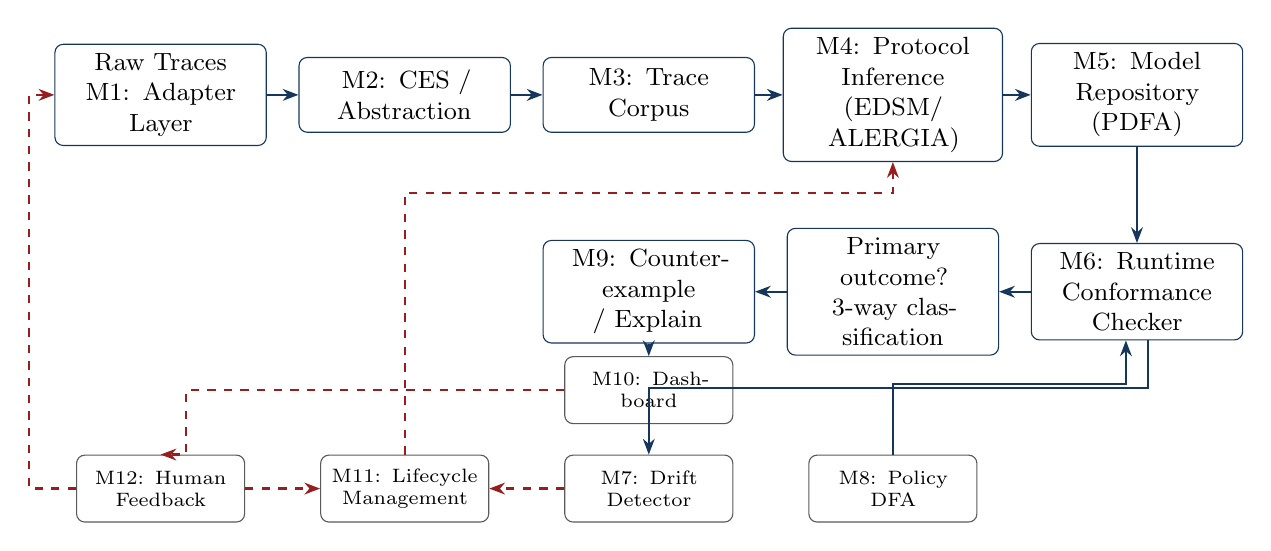
\begin{tikzpicture}[
box/.style={
draw,
rounded corners=3pt,
fill=white,
draw=traceblue,
minimum height=0.95cm,
text width=2.45cm,
align=center,
font=\small
},
small/.style={
draw,
rounded corners=3pt,
fill=white,
draw=tracegray,
minimum height=0.85cm,
text width=1.9cm,
align=center,
font=\scriptsize
},
arrow/.style={
-{Stealth[length=2mm]},
thick,
draw=traceblue
},
farrow/.style={
-{Stealth[length=2mm]},
thick,
draw=nored,
dashed
}
]

\node[box] (m1) at (0,0)
{Raw Traces\\M1: Adapter Layer};

\node[box] (m2) at (3.1,0)
{M2: CES /\\Abstraction};

\node[box] (m3) at (6.2,0)
{M3: Trace\\Corpus};

\node[box, text width=2.55cm] (m4) at (9.3,0)
{M4: Protocol\\Inference\\(EDSM/\allowbreak ALERGIA)};

\node[box] (m5) at (12.4,0)
{M5: Model\\Repository\\(PDFA)};

\node[box] (m9) at (6.2,-2.5)
{M9: Counter-\\example / Explain};

\node[box] (violation) at (9.3,-2.5)
{Primary outcome?\\3-way classification};

\node[box] (m6) at (12.4,-2.5)
{M6: Runtime\\Conformance\\Checker};

\node[small] (m12) at (0,-5.0)
{M12: Human\\Feedback};

\node[small] (m11) at (3.1,-5.0)
{M11: Lifecycle\\Management};

\node[small] (m7) at (6.2,-5.0)
{M7: Drift\\Detector};

\node[small] (m8) at (9.3,-5.0)
{M8: Policy\\DFA};

\node[small] (m10) at (6.2,-3.75)
{M10: Dashboard};

\draw[arrow] (m1.east) -- (m2.west);
\draw[arrow] (m2.east) -- (m3.west);
\draw[arrow] (m3.east) -- (m4.west);
\draw[arrow] (m4.east) -- (m5.west);

\draw[arrow] (m5.south) -- (m6.north);

\draw[arrow] (m6.west) -- (violation.east);
\draw[arrow] (violation.west) -- (m9.east);

\draw[arrow] (m9.south) -- (m10.north);

\draw[arrow] (m8.north) -- ++(0,0.9) -| ([xshift=-4pt]m6.south);

\draw[arrow] ([xshift=4pt]m6.south) -- ++(0,-0.6) -| (m7.north);

\draw[farrow] (m7.west) -- (m11.east);

\draw[farrow] (m10.west) -- ++(-4.8,0) |- (m12.north);

\draw[farrow] (m12.east) -- (m11.west);

\draw[farrow] (m12.west) -- ++(-0.6,0) |- (m1.west);

\draw[farrow] (m11.north) -- (3.1,-1.25) -- (9.3,-1.25) -- (m4.south);

\end{tikzpicture}

\caption{Overall TRACE v2.0 implementation pipeline. Solid blue arrows represent
primary data and verification flow. Dashed red arrows represent feedback and model
lifecycle interactions. M1 contains seven heterogeneous agent-framework adapters and
two benchmark-trajectory adapters. The implementation includes CES validation,
state-merging inference, bounded hierarchical delegation, policy-product verification,
drift monitoring, HITL feedback, API/dashboard interfaces, and model lifecycle handling.}
\label{fig:pipeline}

\end{figure}

\subsection{Runtime Operation (Online Path)}

For each incoming event, the applicable adapter converts source-specific data into the
TRACE event representation. The event is validated against CES v1.0. Recognized secrets
are redacted using entropy- and pattern-based detection before parameter-schema hashing.

The normalized event is then associated with the learned symbolic representation used by
the current behavioral model. The runtime verifier advances the learned behavioral state
and explicit policy state independently while retaining the joint state

\[
(q_A,q_P) \in Q_A \times Q_P.
\]

The primary classification precedence is:

\begin{enumerate}
\item explicit policy violation;
\item structurally unseen transition;
\item low-probability transition;
\item otherwise conformant.
\end{enumerate}

Where multiple conditions are simultaneously present, secondary diagnostic flags may be
retained, but the primary classification follows the above precedence.

This separation ensures that a learned model's statistical normality cannot override an
explicit policy restriction.

\subsection{Learning Operation (Offline Path)}

Canonical symbolic traces are represented as a Prefix Tree Acceptor (PTA). State and
transition evidence is then used by the implemented state-merging inference machinery,
including EDSM ordering and ALERGIA/MDI-style statistical compatibility.

The resulting representation is a probabilistic deterministic finite automaton. The
current documentation does not establish a Hopcroft-style DFA minimization step for this
learned PDFA; therefore no such minimization is asserted here.

The model is stored in a versioned repository and can participate in the implemented
candidate lifecycle.

% ======================================================
\section{Detailed Description of the Invention}
% ======================================================

\subsection{System Architecture (Modules M1--M12)}

TRACE is organized into twelve functional modules. Several modules operate as
cross-cutting services supporting the online verification and model-lifecycle paths.

\begin{longtable}{L{1.7cm} L{4.6cm} L{8.1cm}}
\caption{Module-level architecture summary.}
\label{tab:modules}\\
\toprule
\textbf{Module} & \textbf{Purpose} & \textbf{Implemented Mechanism / Notes} \\
\midrule
\endfirsthead

\toprule
\textbf{Module} & \textbf{Purpose} & \textbf{Implemented Mechanism / Notes} \\
\midrule
\endhead

\bottomrule
\endfoot

\bottomrule
\endlastfoot

M1 &
Trace Ingestion &
Nine active trace adapters comprising seven agent-framework adapters
(MCP, LangGraph, CrewAI, AutoGen/AG2, OpenAI Agents SDK, Semantic Kernel,
Google ADK/Vertex AI) and two benchmark-trajectory adapters (SWE-bench and OSWorld).
\\

M2 &
CES Normalization and Semantic Abstraction &
Canonical Event Schema validation and normalization, including the implemented
secret-redaction mechanism. The repository also defines the semantic-symbol abstraction
architecture; the supplied README does not provide a quantitative ablation establishing
its performance benefit. \\

M3 &
Trace Store / Corpus Management &
SQLite CES relational persistence, trace corpus management, role-specific corpora,
windowing, and trace completeness handling documented by the implementation. \\

M4 &
PTA and Protocol Inference &
Prefix Tree Acceptor construction, ALERGIA/MDI-style statistical state merging,
and EDSM inference machinery. \\

M5 &
Versioned PDFA Model Repository &
Storage and lifecycle management for learned probabilistic models, including
candidate, shadowed, active, and superseded states. No Hopcroft-style PDFA minimization
is asserted. \\

M6 &
Runtime Verification / Product Automaton &
Joint tracking of learned PDFA and explicit policy DFA states with structural,
statistical, and policy classification. \\

M7 &
Behavioral Drift Monitoring &
Rolling conformance/NLL distributions, two-sample KS testing, and tail-quantile
CUSUM monitoring. \\

M8 &
Policy DSL and Policy DFA Compilation &
Declarative policy language and bounded-counter DFA construction for explicit safety and
compliance constraints. \\

M9 &
Counterexample Generation &
Generation of human-readable violation explanations and expected-versus-observed
transition differences. \\

M10 &
Dashboard / Developer Interface &
Implemented web dashboard at \texttt{/dashboard}, including automata visualization,
verification interaction, HITL triage, and benchmark presentation elements documented
by the repository. \\

M11 &
Lifecycle / Relearning Management &
Supports model lifecycle operations and drift-related relearning workflow where
documented by the implementation. The supplied evidence does not establish a universal
automatic scheduling policy for every deployment environment. \\

M12 &
Human-in-the-Loop Feedback / Triage &
Violation triage and candidate model lifecycle support, including feedback recording
and promotion/review mechanisms. \\

\end{longtable}

\subsection{Canonical Event Schema (CES)}

TRACE implements Canonical Event Schema (CES) v1.0 with JSON Schema draft 2020-12
validation. The schema provides a stable representation through which events originating
from structurally different sources can enter the common processing pipeline.

The documented event representation includes fields associated with agent identity,
event type, symbolic action identity, attributes, timestamps, parent-span relationships,
and delegation depth.

The implementation separates event-level categorization from the fine-grained symbolic
representation used by the inference engine. The supplied repository establishes the
CES implementation and validation mechanism, but the README does not provide a complete
quantitative evaluation of the semantic abstraction layer.

\subsection{Secret Redaction}

TRACE implements a secret-redaction mechanism before parameter-schema hashing.

The mechanism combines:

\begin{itemize}
\item entropy-based detection; and
\item pattern/token matching.
\end{itemize}

The documented target classes include API keys, Bearer tokens, private keys, and
authorization headers.

The mechanism should be understood as a mitigation intended to prevent recognized secrets
from entering normalized or hashable parameter representations. The implementation name
``Zero-Leak Secret Redactor'' does not imply a mathematical or universal guarantee of
zero information leakage.

Malformed events failing schema validation can be partitioned into a dead-letter
handling path rather than being admitted into the valid CES store.

\begin{figure}[!htbp]
\centering

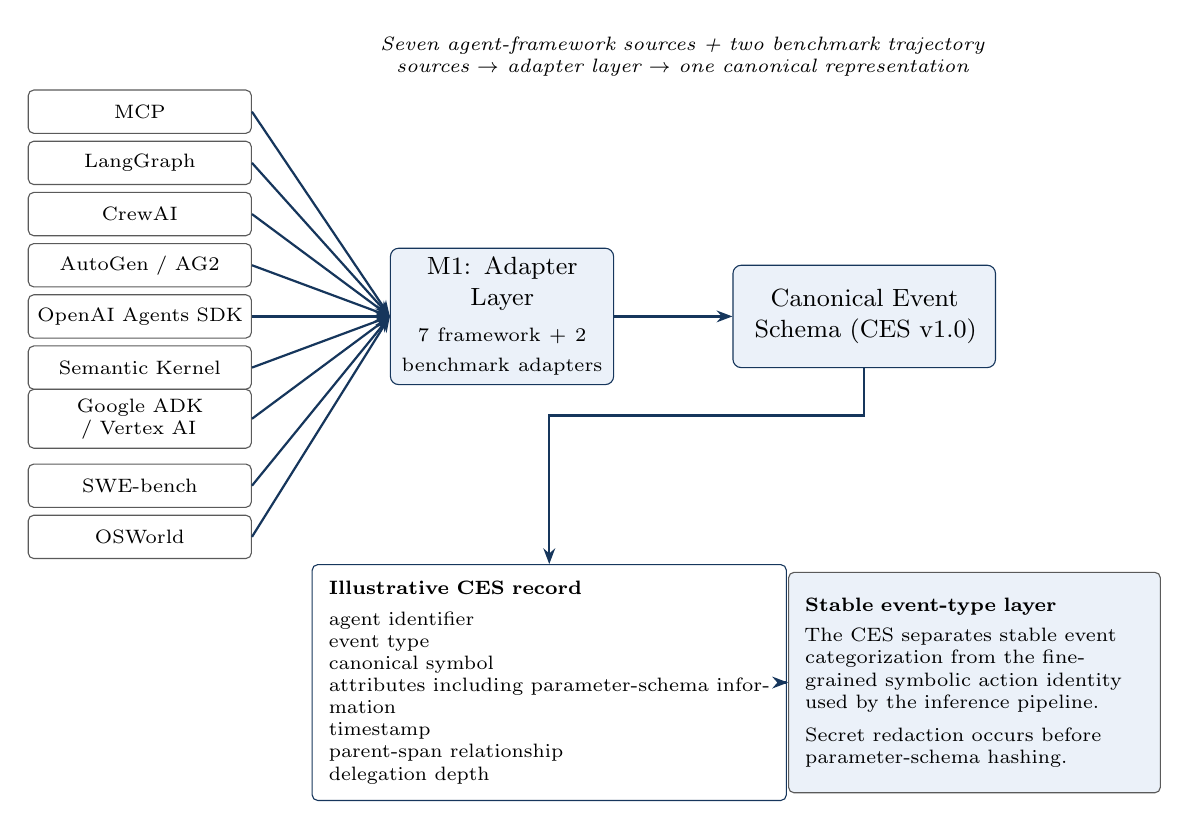
\begin{tikzpicture}[
fw/.style={draw, rounded corners=2pt, fill=white, draw=tracegray,
minimum height=0.55cm, text width=2.6cm, align=center, font=\scriptsize},
hub/.style={draw, rounded corners=3pt, fill=tracelight, draw=traceblue,
minimum height=1.3cm, text width=2.6cm, align=center, font=\small},
card/.style={draw, rounded corners=2pt, fill=white, draw=traceblue,
minimum height=2.8cm, text width=5.6cm, align=left, font=\scriptsize, inner sep=6pt},
taxbox/.style={draw, rounded corners=2pt, fill=tracelight, draw=tracegray,
minimum height=2.8cm, text width=4.3cm, align=left, font=\scriptsize, inner sep=6pt},
arrow/.style={-{Stealth[length=2mm]}, thick, draw=traceblue}
]

\node[fw] (f0) at (0,4.55) {MCP};
\node[fw] (f1) at (0,3.90) {LangGraph};
\node[fw] (f2) at (0,3.25) {CrewAI};
\node[fw] (f3) at (0,2.60) {AutoGen / AG2};
\node[fw] (f4) at (0,1.95) {OpenAI Agents SDK};
\node[fw] (f5) at (0,1.30) {Semantic Kernel};
\node[fw] (f6) at (0,0.65) {Google ADK / Vertex AI};

\node[fw] (b1) at (0,-0.20) {SWE-bench};
\node[fw] (b2) at (0,-0.85) {OSWorld};

\node[hub] (m1) at (4.6,1.95)
{M1: Adapter Layer\\[2pt]
\scriptsize 7 framework + 2 benchmark adapters};

\node[hub, text width=3.1cm] (ces) at (9.2,1.95)
{Canonical Event\\Schema (CES v1.0)};

\draw[arrow] (f0.east) -- (m1.west);
\draw[arrow] (f1.east) -- (m1.west);
\draw[arrow] (f2.east) -- (m1.west);
\draw[arrow] (f3.east) -- (m1.west);
\draw[arrow] (f4.east) -- (m1.west);
\draw[arrow] (f5.east) -- (m1.west);
\draw[arrow] (f6.east) -- (m1.west);
\draw[arrow] (b1.east) -- (m1.west);
\draw[arrow] (b2.east) -- (m1.west);

\draw[arrow] (m1.east) -- (ces.west);

\node[card] (rec) at (5.2,-2.7)
{\textbf{Illustrative CES record}\\[3pt]
agent identifier\\
event type\\
canonical symbol\\
attributes including parameter-schema information\\
timestamp\\
parent-span relationship\\
delegation depth};

\node[taxbox] (tax) at (10.6,-2.7)
{\textbf{Stable event-type layer}\\[3pt]
The CES separates stable event categorization from the fine-grained symbolic
action identity used by the inference pipeline.\\[4pt]
Secret redaction occurs before parameter-schema hashing.};

\draw[arrow] (ces.south) -- ++(0,-0.6) -| (rec.north);
\draw[arrow] (rec.east) -- (tax.west);

\node[font=\scriptsize\itshape, text width=9cm, align=center] at (6.9,5.25)
{Seven agent-framework sources + two benchmark trajectory sources
$\rightarrow$ adapter layer $\rightarrow$ one canonical representation};

\end{tikzpicture}

\caption{Implemented framework adapter and Canonical Event Schema layer. The current
repository documents seven heterogeneous agent-framework adapters and two benchmark
trajectory adapters. Valid events enter the CES pipeline after schema validation and
recognized secret redaction; malformed schema records are handled through the
dead-letter path.}
\label{fig:ces}

\end{figure}

\subsection{Framework Adapters}

The current implementation documents nine active trace adapters:

\begin{enumerate}
\item Model Context Protocol (MCP);
\item LangGraph;
\item CrewAI;
\item AutoGen / AG2;
\item OpenAI Agents SDK;
\item Semantic Kernel;
\item Google ADK / Vertex AI;
\item SWE-bench; and
\item OSWorld.
\end{enumerate}

The first seven are heterogeneous agent-\allowbreak framework adapters.
SWE-\allowbreak bench and OSWorld are benchmark-\allowbreak trajectory adapters
and are not themselves agent frameworks.

This distinction is important because benchmark trajectory importers and live framework
adapters have different source semantics and should not be represented as nine equivalent
framework integrations.

\subsection{Semantic Abstraction}

The architecture describes semantic abstraction of fine-grained action identities using
information such as tool names, documentation, and parameter schemas, potentially
followed by text embeddings, clustering, centroid assignment, and approximate-nearest
neighbor indexing.

The supplied README establishes the existence of the CES normalization and the semantic
abstraction layer in the repository architecture, but it does not provide sufficient
experimental evidence to assert a measured semantic-clustering F1, compression ratio,
cluster purity, or downstream improvement.

Accordingly, this disclosure distinguishes the mechanism from its experimental validation.
Where the implementation exposes semantic action representations, those representations
are part of the implemented system. Claims of quantitative superiority of the semantic
abstraction mechanism remain unsupported by the supplied benchmark results.

\begin{figure}[!htbp]
\centering

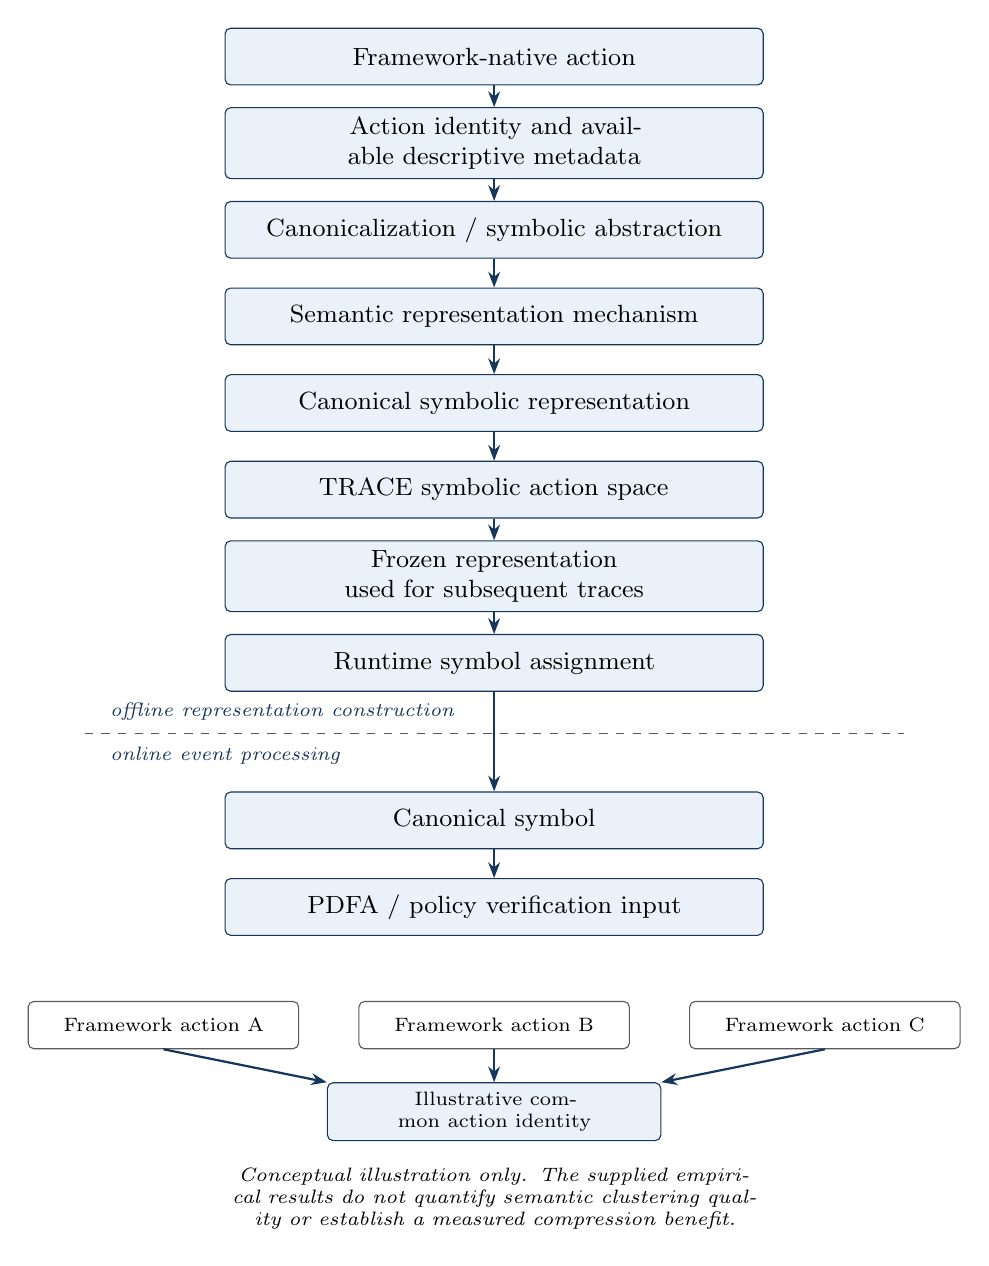
\begin{tikzpicture}[
stg/.style={draw, rounded corners=2pt, fill=tracelight, draw=traceblue,
minimum height=0.72cm, text width=6.6cm, align=center, font=\small},
ex/.style={draw, rounded corners=2pt, fill=white, draw=tracegray,
minimum height=0.6cm, text width=3.2cm, align=center, font=\scriptsize},
tgt/.style={draw, rounded corners=2pt, fill=tracelight, draw=traceblue,
minimum height=0.65cm, text width=4.0cm, align=center, font=\scriptsize},
arrow/.style={-{Stealth[length=2mm]}, thick, draw=traceblue}
]

\node[stg] (s1) at (0,9.9)  {Framework-native action};
\node[stg] (s2) at (0,8.8)  {Action identity and available descriptive metadata};
\node[stg] (s3) at (0,7.7)  {Canonicalization / symbolic abstraction};
\node[stg] (s4) at (0,6.6)  {Semantic representation mechanism};
\node[stg] (s5) at (0,5.5)  {Canonical symbolic representation};
\node[stg] (s6) at (0,4.4)  {TRACE symbolic action space};
\node[stg] (s7) at (0,3.3)  {Frozen representation used for subsequent traces};
\node[stg] (s8) at (0,2.2)  {Runtime symbol assignment};

\draw[dashed, draw=tracegray] (-5.2,1.3) -- (5.2,1.3);
\node[font=\scriptsize\itshape, color=traceblue, anchor=south west] at (-5.0,1.35)
{offline representation construction};
\node[font=\scriptsize\itshape, color=traceblue, anchor=north west] at (-5.0,1.25)
{online event processing};

\node[stg] (s9) at (0,0.2)   {Canonical symbol};
\node[stg] (s10) at (0,-0.9) {PDFA / policy verification input};

\draw[arrow] (s1.south) -- (s2.north);
\draw[arrow] (s2.south) -- (s3.north);
\draw[arrow] (s3.south) -- (s4.north);
\draw[arrow] (s4.south) -- (s5.north);
\draw[arrow] (s5.south) -- (s6.north);
\draw[arrow] (s6.south) -- (s7.north);
\draw[arrow] (s7.south) -- (s8.north);
\draw[arrow] (s8.south) -- (s9.north);
\draw[arrow] (s9.south) -- (s10.north);

\node[ex] (e1) at (-4.2,-2.4) {Framework action A};
\node[ex] (e2) at (0,-2.4)    {Framework action B};
\node[ex] (e3) at (4.2,-2.4)  {Framework action C};
\node[tgt] (tgtn) at (0,-3.5) {Illustrative common action identity};

\draw[arrow] (e1.south) -- (tgtn.north west);
\draw[arrow] (e2.south) -- (tgtn.north);
\draw[arrow] (e3.south) -- (tgtn.north east);

\node[font=\scriptsize\itshape, text width=9.5cm, align=center] at (0,-4.6)
{Conceptual illustration only. The supplied empirical results do not quantify semantic
clustering quality or establish a measured compression benefit.};

\end{tikzpicture}

\caption{Semantic abstraction architecture. The system separates source-specific event
representation from the canonical symbolic representation consumed by the inference
and verification layers. Embedding, clustering, centroid assignment, and ANN mechanisms
described in the architecture should not be interpreted as having a measured benchmark
result unless such a result is explicitly supplied.}
\label{fig:semantic}

\end{figure}

\subsection{Protocol Inference}

The implemented inference path constructs a Prefix Tree Acceptor from symbolic traces and
uses state-merging mechanisms including EDSM and ALERGIA/MDI-style statistical
compatibility.

RPNI is not asserted as the principal TRACE inference mechanism and is not claimed as
inventive. The primary implemented machinery is based on probabilistic state merging and
EDSM-style inference.

The resulting representation is a probabilistic deterministic finite automaton (PDFA).
No unsupported claim of Hopcroft-style minimization is made.

\begin{figure}[!htbp]
\centering

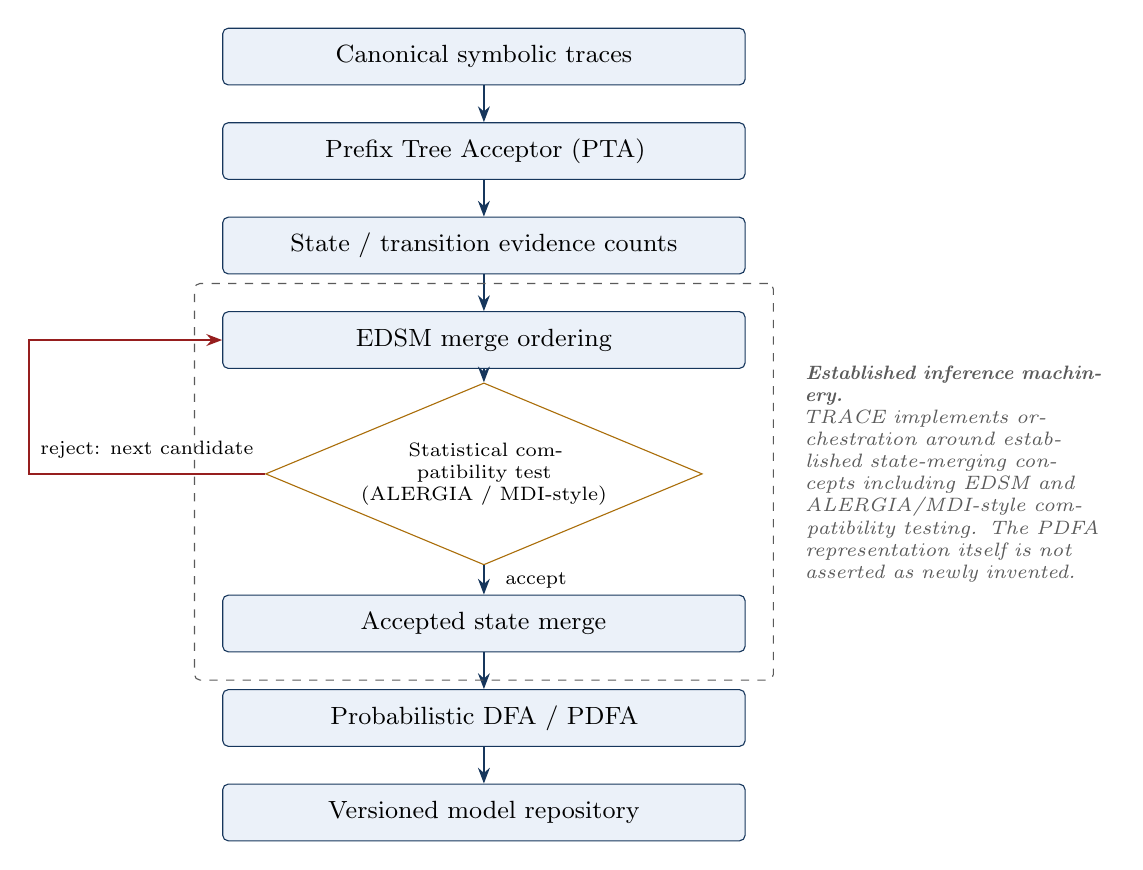
\begin{tikzpicture}[
stg/.style={draw, rounded corners=2pt, fill=tracelight, draw=traceblue,
minimum height=0.72cm, text width=6.4cm, align=center, font=\small},
dec/.style={draw, diamond, aspect=2.4, fill=white, draw=partialorange,
text width=3.4cm, align=center, font=\scriptsize, inner sep=1pt},
note/.style={font=\scriptsize\itshape, color=tracegray, align=left, text width=3.8cm},
arrow/.style={-{Stealth[length=2mm]}, thick, draw=traceblue},
rarrow/.style={-{Stealth[length=2mm]}, thick, draw=nored}
]

\node[stg] (i1) at (0,8.5) {Canonical symbolic traces};
\node[stg] (i2) at (0,7.3) {Prefix Tree Acceptor (PTA)};
\node[stg] (i3) at (0,6.1) {State / transition evidence counts};
\node[stg] (i4) at (0,4.9) {EDSM merge ordering};
\node[dec] (i5) at (0,3.2)
{Statistical compatibility test\\
(ALERGIA / MDI-style)};
\node[stg] (i6) at (0,1.3) {Accepted state merge};
\node[stg] (i7) at (0,0.1) {Probabilistic DFA / PDFA};
\node[stg] (i8) at (0,-1.1) {Versioned model repository};

\draw[arrow] (i1.south) -- (i2.north);
\draw[arrow] (i2.south) -- (i3.north);
\draw[arrow] (i3.south) -- (i4.north);
\draw[arrow] (i4.south) -- (i5.north);
\draw[arrow] (i5.south) -- node[right=4pt,font=\scriptsize]{accept} (i6.north);
\draw[arrow] (i6.south) -- (i7.north);
\draw[arrow] (i7.south) -- (i8.north);

\draw[rarrow]
(i5.west) -- node[above=2pt,font=\scriptsize]
{reject: next candidate}
++(-3.0,0) |- (i4.west);

\node[dashed, draw=tracegray, rounded corners=2pt,
fit=(i4)(i5)(i6), inner sep=10pt] {};

\node[note] at (6.0,3.2)
{\textbf{Established inference machinery.}\\
TRACE implements orchestration around established state-merging concepts including
EDSM and ALERGIA/MDI-style compatibility testing. The PDFA representation itself is
not asserted as newly invented.};

\end{tikzpicture}

\caption{Implemented probabilistic automata inference pipeline. Canonical symbolic
traces are converted into a PTA, candidate state merges are ordered using EDSM-style
evidence, compatibility is evaluated using ALERGIA/MDI-style statistical criteria, and
accepted merges produce a probabilistic finite-state behavioral model. The current
disclosure does not assert Hopcroft-style minimization of the learned PDFA.}
\label{fig:inference}

\end{figure}

\subsection{Hierarchical Trace Folding}

The implementation represents multi-agent delegation using role-specific corpora and
explicit delegation boundaries.

The documented implementation includes:

\begin{itemize}
\item \texttt{delegate(role)} boundary symbols;
\item parent and child trace relationships;
\item role-specific corpora;
\item \texttt{parent\_span\_id} linkage;
\item orphan-span / missing-child handling; and
\item \texttt{MAX\_DELEGATION\_DEPTH = 8}.
\end{itemize}

The implementation therefore uses bounded hierarchical composition. It does not establish
support for unbounded recursion or a general pushdown automaton.

\begin{figure}[!htbp]
\centering

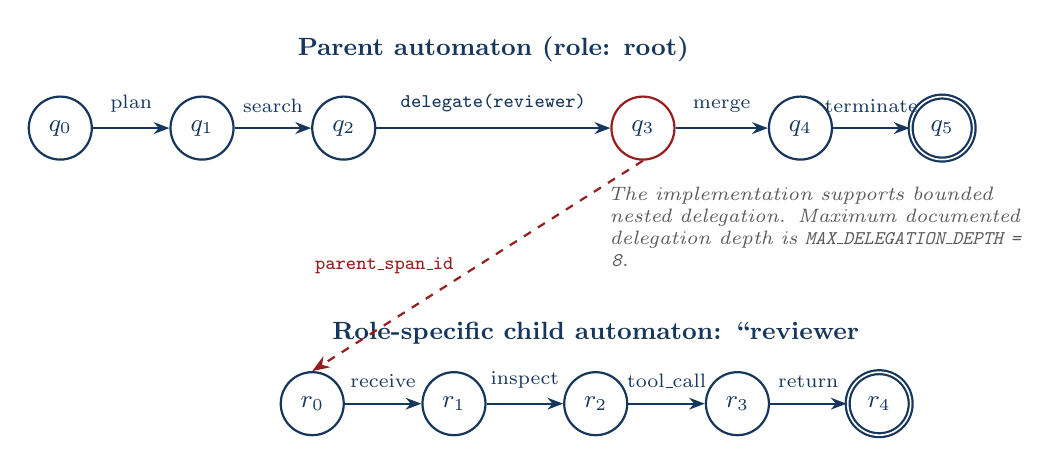
\begin{tikzpicture}[
st/.style={
draw,
circle,
minimum size=0.8cm,
inner sep=0pt,
color=traceblue,
thick,
font=\small
},
lab/.style={
font=\small\bfseries,
color=traceblue
},
edge/.style={
-{Stealth[length=2mm]},
thick,
color=traceblue
}
]

\node[lab] at (5.5,2.7)
{\textbf{Parent automaton (role: root)}};

\node[st] (p0) at (0,1.7) {$q_0$};
\node[st] (p1) at (1.8,1.7) {$q_1$};
\node[st] (p2) at (3.6,1.7) {$q_2$};
\node[st,draw=nored,thick] (p3) at (7.4,1.7) {$q_3$};
\node[st] (p4) at (9.4,1.7) {$q_4$};
\node[st,double] (p5) at (11.2,1.7) {$q_5$};

\draw[edge]
(p0) -- node[above=2pt,font=\scriptsize]{plan} (p1);

\draw[edge]
(p1) -- node[above=2pt,font=\scriptsize]{search} (p2);

\draw[edge]
(p2) -- node[above=2pt,font=\scriptsize\ttfamily]
{delegate(reviewer)} (p3);

\draw[edge]
(p3) -- node[above=2pt,font=\scriptsize]{merge} (p4);

\draw[edge]
(p4) -- node[above=2pt,font=\scriptsize]{terminate} (p5);

\node[lab] at (6.8,-0.9)
{\textbf{Role-specific child automaton: ``reviewer}};

\node[st] (c0) at (3.2,-1.8) {$r_0$};
\node[st] (c1) at (5.0,-1.8) {$r_1$};
\node[st] (c2) at (6.8,-1.8) {$r_2$};
\node[st] (c3) at (8.6,-1.8) {$r_3$};
\node[st,double] (c4) at (10.4,-1.8) {$r_4$};

\draw[edge]
(c0) -- node[above=2pt,font=\scriptsize]{receive} (c1);

\draw[edge]
(c1) -- node[above=2pt,font=\scriptsize]{inspect} (c2);

\draw[edge]
(c2) -- node[above=2pt,font=\scriptsize]{tool\_call} (c3);

\draw[edge]
(c3) -- node[above=2pt,font=\scriptsize]{return} (c4);

\draw[
-{Stealth[length=2.2mm]},
thick,
color=nored,
dashed
]
(p3.south)
-- node[midway,left=5pt,font=\scriptsize\ttfamily,color=nored]
{parent\_span\_id} (c0.north);

\node[font=\scriptsize\itshape, text width=5.2cm, align=left, color=tracegray]
at (9.6,0.45)
{The implementation supports bounded nested delegation. Maximum documented delegation depth is \texttt{MAX\_DELEGATION\_DEPTH = 8}.};

\end{tikzpicture}

\caption{Hierarchical delegation representation. A parent trace retains a
\texttt{delegate(role)} boundary while the delegated execution is represented using a
role-specific child corpus and automaton linked through trace-span information. The
implementation uses bounded-depth hierarchical composition and does not claim unbounded
pushdown-automaton semantics.}
\label{fig:hierarchy}

\end{figure}

Mathematically, the parent language remains regular over an alphabet containing
\texttt{delegate(role)} as an atomic symbol. A role-specific child automaton is associated
with the delegation boundary rather than expanded into the parent state machine.

This provides a bounded hierarchical representation while avoiding the claim that TRACE
models arbitrary unbounded call-stack behavior.

\subsection{Runtime Verification and the Product Automaton}

The learned behavioral model is represented as

\[
A=(Q_A,\Sigma,\delta_A,q_{A0},P_A),
\]

where $Q_A$ is the learned state set, $\Sigma$ is the canonical symbolic alphabet,
$\delta_A$ is the learned transition function, $q_{A0}$ is the initial state, and
$P_A$ represents transition probabilities.

The explicit policy DFA is represented as

\[
P=(Q_P,\Sigma,\delta_P,q_{P0},F_P),
\]

where $Q_P$ is the policy-state set, $\delta_P$ is the deterministic policy transition
function, $q_{P0}$ is the policy initial state, and $F_P$ represents its accepting
states.

The verifier tracks

\[
(q_A,q_P)\in Q_A\times Q_P.
\]

The learned and policy components are evaluated independently.

\begin{figure}[!htbp]
\centering

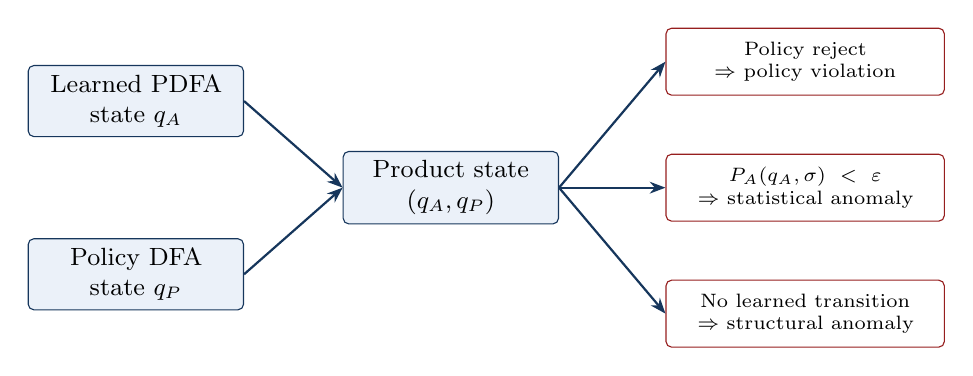
\begin{tikzpicture}[
box/.style={draw, rounded corners=2pt, fill=tracelight, draw=traceblue,
minimum height=0.85cm, text width=2.5cm, align=center, font=\small},
outbox/.style={draw, rounded corners=2pt, fill=white, draw=nored,
minimum height=0.85cm, text width=3.3cm, align=center, font=\scriptsize},
arrow/.style={-{Stealth[length=2mm]}, thick, draw=traceblue}
]

\node[box] (a) at (0,1.1)  {Learned PDFA\\state $q_A$};
\node[box] (p) at (0,-1.1) {Policy DFA\\state $q_P$};

\node[box] (prod) at (4.0,0) {Product state\\$(q_A,q_P)$};

\node[outbox] (o1) at (8.5,1.6)
{Policy reject\\$\Rightarrow$ policy violation};

\node[outbox] (o2) at (8.5,0)
{$P_A(q_A,\sigma)<\varepsilon$\\
$\Rightarrow$ statistical anomaly};

\node[outbox] (o3) at (8.5,-1.6)
{No learned transition\\$\Rightarrow$ structural anomaly};

\draw[arrow] (a.east) -- (prod.west);
\draw[arrow] (p.east) -- (prod.west);

\draw[arrow] (prod.east) -- (o1.west);
\draw[arrow] (prod.east) -- (o2.west);
\draw[arrow] (prod.east) -- (o3.west);

\end{tikzpicture}

\caption{Product-state runtime verification. The learned probabilistic model and
explicit policy DFA are evaluated independently while the verifier tracks their joint
state. Explicit policy violations take precedence over learned statistical conditions;
structural and statistical anomaly signals are retained as separate diagnostic classes.}
\label{fig:product}

\end{figure}

The primary classification precedence is:

\begin{enumerate}
\item \textbf{Policy violation}: the observed transition violates the explicit policy
DFA.
\item \textbf{Structural anomaly}: the transition is not represented as an observed
transition from the current learned state.
\item \textbf{Statistical anomaly}: the transition exists but its learned probability
falls below the configured threshold $\varepsilon$.
\item \textbf{Conformant}: none of the above conditions applies.
\end{enumerate}

The verifier may retain secondary flags when more than one condition is diagnostically
relevant.

This is runtime verification of an observed execution. It is not exhaustive model
checking of every possible execution path.

\subsection{Counterexample Generation}

The implemented explainability mechanism produces human-readable differences associated
with detected deviations.

A violation explanation can identify the relevant unexpected transition and provide
expected-versus-observed information rather than exposing only raw execution logs.

\begin{figure}[!htbp]
\centering

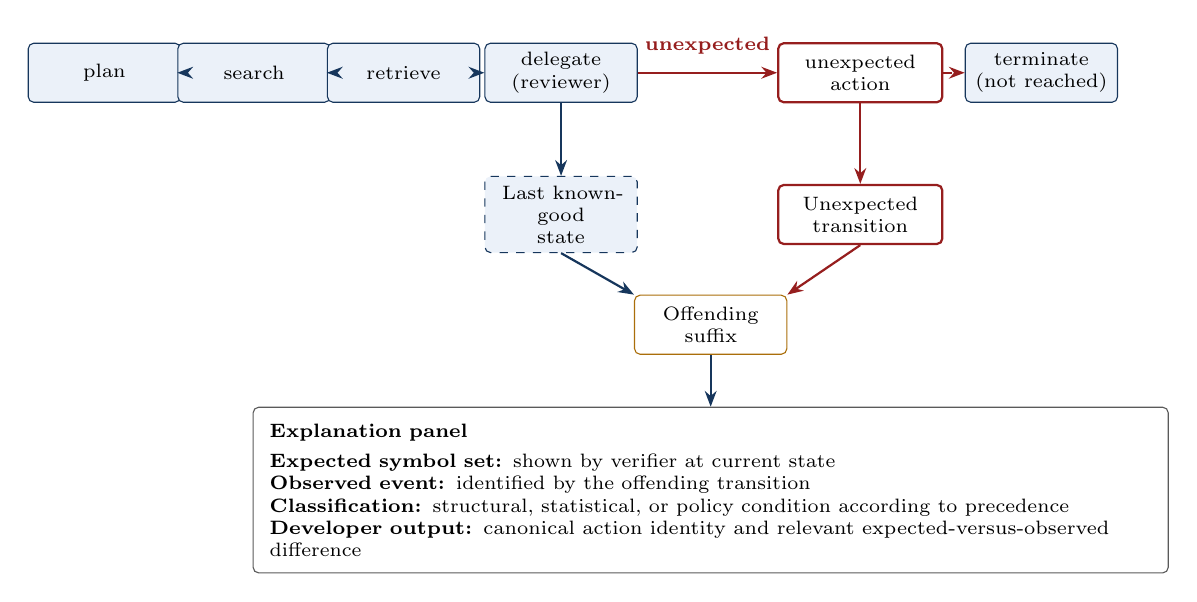
\begin{tikzpicture}[
st/.style={draw, rounded corners=2pt, fill=tracelight, draw=traceblue,
minimum height=0.75cm, text width=1.70cm, align=center, font=\scriptsize},
bad/.style={draw, rounded corners=2pt, fill=white, draw=nored, thick,
minimum height=0.75cm, text width=1.85cm, align=center, font=\scriptsize},
panel/.style={draw, rounded corners=2pt, fill=white, draw=tracegray,
text width=11.2cm, align=left, font=\scriptsize, inner sep=6pt},
arrow/.style={-{Stealth[length=2mm]}, thick, draw=traceblue},
rarrow/.style={-{Stealth[length=2mm]}, thick, draw=nored}
]

\node[st] (t1) at (0,0)     {plan};
\node[st] (t2) at (1.9,0)   {search};
\node[st] (t3) at (3.8,0)   {retrieve};
\node[st] (t4) at (5.8,0)   {delegate\\(reviewer)};
\node[bad] (t5) at (9.6,0)  {unexpected\\action};
\node[st] (t6) at (11.9,0)  {terminate\\(not reached)};

\draw[arrow] (t1.east) -- (t2.west);
\draw[arrow] (t2.east) -- (t3.west);
\draw[arrow] (t3.east) -- (t4.west);
\draw[rarrow] (t4.east) -- node[above=3pt,font=\scriptsize\bfseries,color=nored]{unexpected} (t5.west);
\draw[rarrow, dashed] (t5.east) -- (t6.west);

\node[st, dashed] (lkg) at (5.8,-1.8) {Last known-good\\state};
\node[bad] (ut) at (9.6,-1.8) {Unexpected\\transition};
\node[st, fill=white, draw=partialorange] (suf) at (7.7,-3.2) {Offending\\suffix};

\draw[arrow] (t4.south) -- (lkg.north);
\draw[rarrow] (t5.south) -- (ut.north);
\draw[arrow] (lkg.south) -- (suf.north west);
\draw[rarrow] (ut.south) -- (suf.north east);

\node[panel] (exp) at (7.7,-5.3)
{\textbf{Explanation panel}\\[3pt]
\textbf{Expected symbol set:} shown by verifier at current state\\
\textbf{Observed event:} identified by the offending transition\\
\textbf{Classification:} structural, statistical, or policy condition according to precedence\\
\textbf{Developer output:} canonical action identity and relevant expected-versus-observed difference};

\draw[arrow] (suf.south) -- (exp.north);

\end{tikzpicture}

\caption{Conceptual counterexample explanation. The verifier identifies the relevant
last-known-good state and the offending transition, after which the explainability layer
produces an expected-versus-observed diagnostic. The example is illustrative and is not
a benchmark result.}
\label{fig:counterexample}

\end{figure}

\subsection{Drift Detection}

The implementation includes behavioral drift monitoring based on rolling conformance
statistics.

The supplied README documents two complementary mechanisms:

\begin{enumerate}
\item a two-sample Kolmogorov--Smirnov (KS) test over shifted trace distributions; and
\item tail-quantile CUSUM monitoring.
\end{enumerate}

The system therefore does not treat KS as merely a future proposal. The current
implementation includes the KS and tail-quantile CUSUM mechanisms.

The supplied empirical result for RQ5 is:

\[
\mathrm{KS}=0.9800,\qquad \text{triggered}.
\]

This demonstrates the reported benchmark condition, but does not establish
universal drift-\allowbreak detection accuracy, false-\allowbreak positive rate,
detection latency, or performance across arbitrary non-\allowbreak stationary workloads.

\begin{figure}[!htbp]
\centering

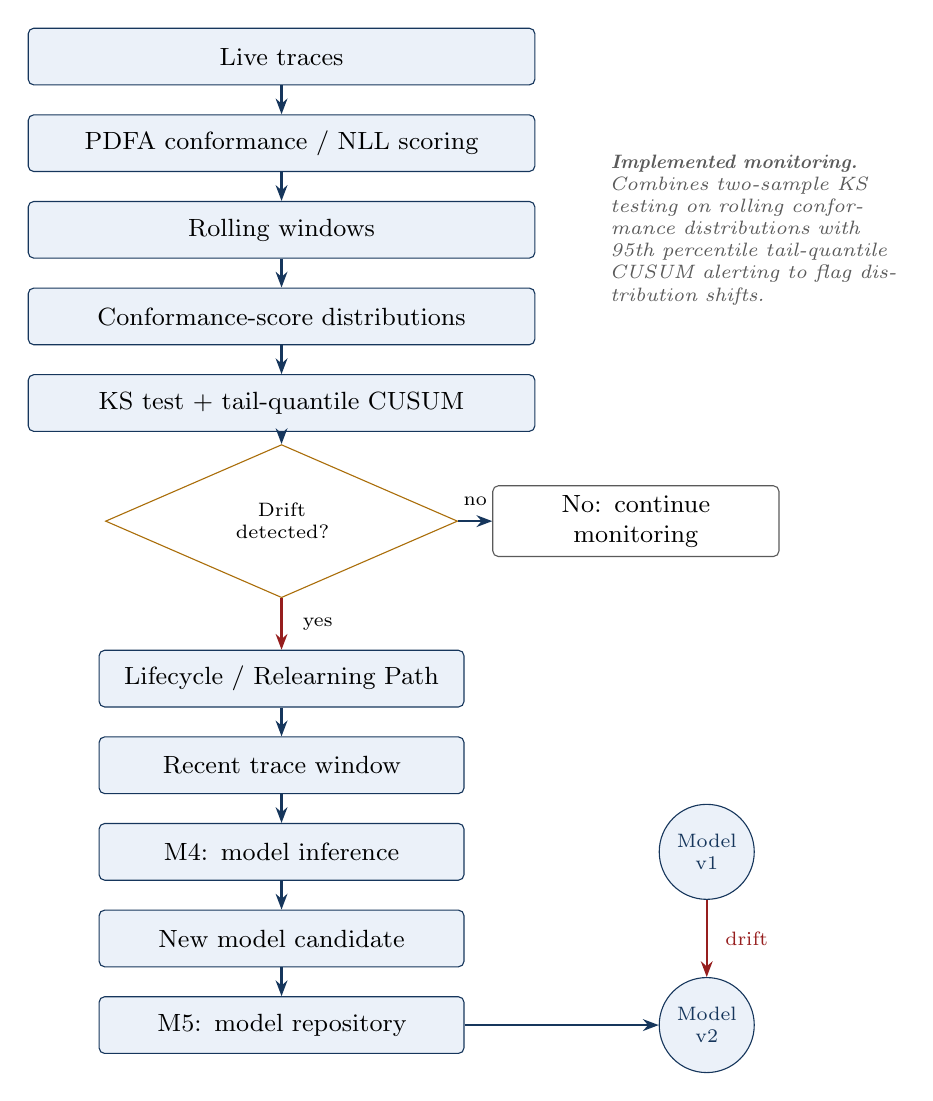
\begin{tikzpicture}[
stg/.style={draw, rounded corners=2pt, fill=tracelight, draw=traceblue,
minimum height=0.72cm, text width=6.2cm, align=center, font=\small},
dec/.style={draw, diamond, aspect=2.3, fill=white, draw=partialorange,
text width=3.2cm, align=center, font=\scriptsize, inner sep=1pt},
note/.style={font=\scriptsize\itshape, color=tracegray, align=left, text width=3.6cm},
arrow/.style={-{Stealth[length=2mm]}, thick, draw=traceblue},
rarrow/.style={-{Stealth[length=2mm]}, thick, draw=nored},
circ/.style={draw, circle, minimum size=1.0cm, color=traceblue, fill=tracelight, font=\scriptsize, align=center}
]

\node[stg] (d1) at (0,7.8) {Live traces};
\node[stg] (d2) at (0,6.7) {PDFA conformance / NLL scoring};
\node[stg] (d3) at (0,5.6) {Rolling windows};
\node[stg] (d4) at (0,4.5) {Conformance-score distributions};
\node[stg] (d5) at (0,3.4) {KS test + tail-quantile CUSUM};

\node[dec] (drift) at (0,1.9) {Drift\\detected?};
\node[stg, draw=tracegray, fill=white, text width=3.4cm] (nom) at (4.5,1.9)
{No: continue\\monitoring};

\node[stg, text width=4.4cm] (relearn) at (0,-0.1) {Lifecycle / Relearning Path};
\node[stg, text width=4.4cm] (win) at (0,-1.2)     {Recent trace window};
\node[stg, text width=4.4cm] (m4) at (0,-2.3)      {M4: model inference};
\node[stg, text width=4.4cm] (cand) at (0,-3.4)    {New model candidate};
\node[stg, text width=4.4cm] (m5) at (0,-4.5)      {M5: model repository};

\node[circ] (mv1) at (5.4,-2.3) {Model\\v1};
\node[circ] (mv2) at (5.4,-4.5) {Model\\v2};

\draw[arrow] (d1.south) -- (d2.north);
\draw[arrow] (d2.south) -- (d3.north);
\draw[arrow] (d3.south) -- (d4.north);
\draw[arrow] (d4.south) -- (d5.north);
\draw[arrow] (d5.south) -- (drift.north);

\draw[arrow] (drift.east) -- node[above=2pt,font=\scriptsize]{no} (nom.west);
\draw[rarrow] (drift.south) -- node[right=4pt,font=\scriptsize]{yes} (relearn.north);

\draw[arrow] (relearn.south) -- (win.north);
\draw[arrow] (win.south) -- (m4.north);
\draw[arrow] (m4.south) -- (cand.north);
\draw[arrow] (cand.south) -- (m5.north);

\draw[rarrow] (mv1.south) -- node[right=3pt,font=\scriptsize,color=nored]{drift} (mv2.north);
\draw[arrow] (m5.east) -- (mv2.west);

\node[note] at (6.0,5.6)
{\textbf{Implemented monitoring.}\\
Combines two-sample KS testing on rolling conformance distributions with 95th percentile
tail-quantile CUSUM alerting to flag distribution shifts.};

\end{tikzpicture}

\caption{Behavioral drift monitoring. Rolling conformance distributions are evaluated
using the implemented KS and tail-quantile CUSUM mechanisms. A detected shift can enter
the model lifecycle/relearning path. The reported RQ5 benchmark demonstrates a triggered
KS result but does not constitute a universal drift-detection guarantee.}
\label{fig:drift}

\end{figure}

\subsection{Computational Complexity}

\begin{table}[!htbp]
\centering
\small
\begin{tabular}{L{4.6cm} L{9.2cm}}
\toprule
\textbf{Module} & \textbf{Complexity / Consideration} \\
\midrule

M1 Ingestion &
$O(n)$ in trace length for per-event parsing, subject to source-specific parser costs. \\

M2 Semantic abstraction &
Embedding and representation costs depend on corpus size and representation dimension.
If nearest-centroid or ANN lookup is used, practical runtime depends on the selected
index structure. \\

M4 State-merging inference &
State merging can have substantial computational cost and does not receive a universal
polynomial-time guarantee from the practical EDSM/ALERGIA-style search process. \\

M6 Runtime verification &
Direct transition lookup can provide effectively constant-time state advancement per
event for the active product state. A fully materialized product has worst-case state
space $O(|Q_A||Q_P|)$, while lazy evaluation can use less space. \\

M7 Drift monitoring &
Window-based statistical monitoring depends on the selected window size and test
implementation and is ordinarily evaluated periodically rather than requiring the full
window computation on every event. \\

\bottomrule
\end{tabular}

\caption{Module-level computational considerations. The measured RQ3 latency is a
verification-engine benchmark result and should not be interpreted as a statement that
the entire end-to-end agent/tool/network interaction has the same latency.}
\end{table}

\subsection{Security and Failure Modes}

\subsubsection*{Implemented Mitigations}

\begin{itemize}[leftmargin=1.4em]

\item \textbf{Secret redaction:} entropy- and pattern-based recognition of documented
secret classes before parameter-schema hashing.

\item \textbf{Schema validation:} CES v1.0 JSON Schema draft 2020-12 validation.

\item \textbf{Dead-letter handling:} malformed or invalid schema records can be separated
from the valid processing path.

\item \textbf{Policy validation:} explicit policy compilation and validation mechanisms.

\item \textbf{Bounded delegation depth:}
\texttt{MAX\_DELEGATION\_DEPTH = 8} limits hierarchical nesting in the current
implementation.

\end{itemize}

\subsubsection*{Remaining Risks}

\begin{itemize}[leftmargin=1.4em]

\item \textbf{Poisoned training traces:} an attacker able to inject malicious or
misleading traces into model-building data could influence the learned behavioral model.
The supplied implementation does not establish a complete training-data-poisoning
defense.

\item \textbf{Semantic over-clustering:} distinct actions may be mapped to insufficiently
distinct symbolic representations, potentially masking a behavioral difference.

\item \textbf{Semantic under-clustering:} excessively fragmented symbolic representations
can increase alphabet size and complicate inference.

\item \textbf{Adversarial tool naming:} malicious tools could attempt to exploit semantic
similarity with trusted actions.

\item \textbf{Model staleness:} drift monitoring provides a mechanism for identifying
distribution changes, but the supplied evidence does not establish general robustness
against all forms of model or workload evolution.

\item \textbf{Incomplete traces:} truncated or missing events can affect learned state
transitions and conformance interpretation.

\item \textbf{Rare legitimate behavior:} legitimate but uncommon actions may be classified
as statistically anomalous.

\item \textbf{Policy conflicts:} contradictory or overly restrictive policy rules may
produce undesired policy states and require policy validation.

\item \textbf{Deployment-\allowbreak scale performance:} the reported latency benchmark does not
establish production-\allowbreak scale performance under arbitrary concurrent agent workloads.

\item \textbf{Adversarial evasion:} the current evidence does not establish robustness
against an attacker deliberately optimizing behavior to remain inside the learned
behavioral distribution.

\end{itemize}

\subsection{End-to-End Operational Swimlane}

Figure~\ref{fig:swimlane} separates the per-event runtime path from the feedback and
model-lifecycle path.

\begin{landscape}
\begin{figure}[p]
\centering

\resizebox{0.97\linewidth}{!}{%
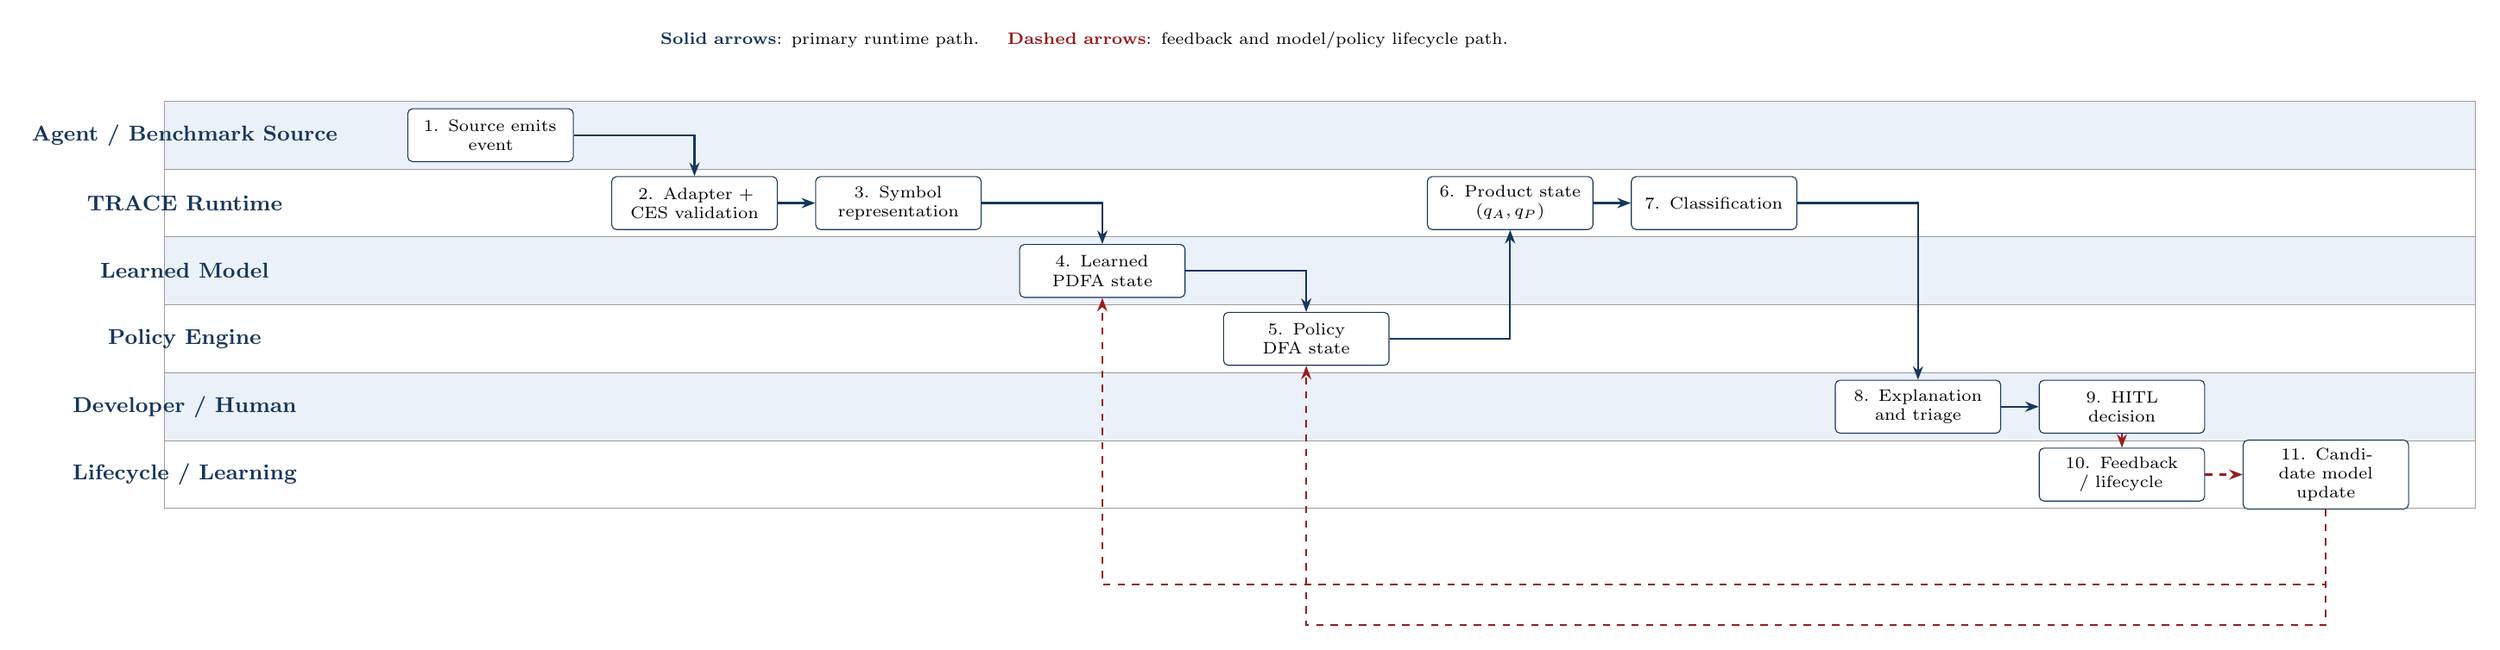
\begin{tikzpicture}[
lane/.style={font=\small\bfseries, color=traceblue, align=left},
stepbox/.style={draw, rounded corners=2pt, fill=white, draw=traceblue,
minimum height=0.78cm, text width=2.2cm, align=center, font=\scriptsize},
arrow/.style={-{Stealth[length=2mm]}, thick, draw=traceblue},
farrow/.style={-{Stealth[length=2mm]}, thick, draw=nored, dashed}
]

\foreach \y/\c in {5/tracelight, 4/white, 3/tracelight, 2/white, 1/tracelight, 0/white} {
\draw[fill=\c, draw=tracegray!60] (-4.8,\y-0.5) rectangle (29.2,\y+0.5);
}

\node[lane] at (-4.5,5) {Agent / Benchmark Source};
\node[lane] at (-4.5,4) {TRACE Runtime};
\node[lane] at (-4.5,3) {Learned Model};
\node[lane] at (-4.5,2) {Policy Engine};
\node[lane] at (-4.5,1) {Developer / Human};
\node[lane] at (-4.5,0) {Lifecycle / Learning};

\node[stepbox] (p1) at (0,5)   {1. Source emits\\event};
\node[stepbox] (p2) at (3,4)   {2. Adapter +\\CES validation};
\node[stepbox] (p3) at (6,4)   {3. Symbol\\representation};
\node[stepbox] (p4) at (9,3)   {4. Learned\\PDFA state};
\node[stepbox] (p5) at (12,2)  {5. Policy\\DFA state};
\node[stepbox] (p6) at (15,4)  {6. Product state\\$(q_A,q_P)$};
\node[stepbox] (p7) at (18,4)  {7. Classification};
\node[stepbox] (p8) at (21,1)  {8. Explanation\\and triage};
\node[stepbox] (p9) at (24,1)  {9. HITL\\decision};
\node[stepbox] (p10) at (24,0) {10. Feedback\\/ lifecycle};
\node[stepbox] (p11) at (27,0) {11. Candidate model\\update};

\draw[arrow] (p1.east) -| (p2.north);
\draw[arrow] (p2.east) -- (p3.west);
\draw[arrow] (p3.east) -| (p4.north);
\draw[arrow] (p4.east) -| (p5.north);
\draw[arrow] (p5.east) -| (p6.south);
\draw[arrow] (p6.east) -- (p7.west);
\draw[arrow] (p7.east) -| (p8.north);
\draw[arrow] (p8.east) -- (p9.west);
\draw[farrow] (p9.south) -- (p10.north);
\draw[farrow] (p10.east) -- (p11.west);

\draw[farrow] (p11.south) -- ++(0,-1.1) -| (p4.south);
\draw[farrow] (p11.south) -- ++(0,-1.7) -| (p5.south);

\node[font=\scriptsize, align=left, text width=15cm] at (10,6.4)
{\textcolor{traceblue}{\textbf{Solid arrows}}: primary runtime path.
\quad
\textcolor{nored}{\textbf{Dashed arrows}}: feedback and model/policy lifecycle path.};

\end{tikzpicture}%
}

\caption{End-to-end operational workflow. A source event enters through an adapter and
CES validation, is converted into the symbolic representation consumed by the learned
and policy tracks, and is evaluated using the joint product state. Deviations can enter
HITL triage and the model/policy lifecycle. The figure describes the implemented
architecture and does not imply that every deployment automatically performs every
lifecycle action.}
\label{fig:swimlane}

\end{figure}
\end{landscape}

\subsection{Operational Interfaces and Deployment}

The current implementation provides the following documented interfaces.

\subsubsection*{FastAPI}

The FastAPI service exposes:

\begin{itemize}
\item \texttt{/v1/events} for event ingestion;
\item \texttt{/v1/verify} for verification;
\item \texttt{/dashboard} for the web console; and
\item \texttt{/metrics} for Prometheus telemetry.
\end{itemize}

\subsubsection*{Dashboard}

The dashboard provides an interactive interface for documented TRACE capabilities,
including automata visualization, verification interaction, HITL triage, and benchmark
presentation.

\subsubsection*{CLI and REPL}

The implementation provides an interactive \texttt{trace} shell and commands for adapter
inspection, policy validation, ingestion, model training, model inspection, validation,
promotion, replay, verification, feedback, and benchmark execution.

The repository documents a 14-step demonstration accessible through:

\begin{verbatim}
trace demo
\end{verbatim}

or non-interactively through:

\begin{verbatim}
trace demo --auto
\end{verbatim}

\subsubsection*{Containerization}

Docker and Docker Compose deployment are documented for the API service.

\subsection{Recommended Patent Drawing Set}

\begin{table}[!htbp]
\centering
\small
\begin{tabular}{L{1.8cm} L{12.3cm}}
\toprule
\textbf{Figure} & \textbf{Content} \\
\midrule

Fig.~\ref{fig:pipeline} &
Overall TRACE implementation architecture and closed-loop pipeline. \\

Fig.~\ref{fig:ces} &
Seven framework adapters plus two benchmark trajectory adapters feeding CES v1.0. \\

Fig.~\ref{fig:semantic} &
Semantic abstraction architecture, explicitly identified as an architectural mechanism
without unsupported quantitative performance claims. \\

Fig.~\ref{fig:inference} &
PTA construction, EDSM ordering, ALERGIA/MDI-style compatibility, state merging, and
PDFA repository. \\

Fig.~\ref{fig:hierarchy} &
Bounded hierarchical delegation with role-specific child automata. \\

Fig.~\ref{fig:product} &
Learned PDFA and explicit policy DFA tracked through a joint product state. \\

Fig.~\ref{fig:counterexample} &
Counterexample and expected-versus-observed explanation flow. \\

Fig.~\ref{fig:drift} &
Implemented KS and tail-quantile CUSUM drift monitoring and lifecycle path. \\

Fig.~\ref{fig:swimlane} &
End-to-end runtime and feedback/lifecycle workflow. \\

\bottomrule
\end{tabular}

\caption{Recommended figure set for formal patent-drawing preparation.}
\end{table}

% ======================================================
\section{Experimental Validation Results}
% ======================================================

\subsection{Current Implementation Status}

The supplied repository README establishes that TRACE v2.0 is an implemented software
prototype rather than a concept-only architecture.

The documented implementation includes:

\begin{itemize}
\item nine active trace adapters;
\item CES v1.0 and JSON Schema draft 2020-12 validation;
\item entropy- and pattern-based secret redaction;
\item dead-letter handling;
\item SQLite persistence;
\item PTA construction;
\item ALERGIA/MDI-style state merging;
\item EDSM;
\item PDFA representation;
\item bounded hierarchical delegation;
\item policy DSL and DFA compilation;
\item product-automaton runtime verification;
\item structural, statistical, and policy anomaly classification;
\item running NLL scoring;
\item counterexample explanation;
\item KS and tail-quantile CUSUM drift monitoring;
\item HITL triage and model lifecycle;
\item FastAPI endpoints;
\item dashboard;
\item Prometheus telemetry;
\item Docker and Docker Compose;
\item interactive CLI and REPL;
\item 14-step capability demonstration; and
\item empirical benchmark execution infrastructure.
\end{itemize}

The repository additionally documents 57 automated software tests with a 100\% pass
rate.

The 57 automated tests should not be conflated with scientific validation of the
research questions. Software tests establish that the tested implementation contracts
and fixtures pass under the test suite. The empirical benchmark results described below
address separate research questions.

\subsection{Automated Testing Evidence}

The documented automated test matrix is:

\begin{table}[!htbp]
\centering
\small
\begin{tabular}{L{5.2cm} L{5.8cm} C{1.4cm} C{2.0cm}}
\toprule
\textbf{Test Suite} & \textbf{Target Layer} & \textbf{Tests} & \textbf{Result} \\
\midrule
Adapters & Seven core framework adapters & 8 & Passed \\
Benchmark & SWE-bench and OSWorld importers & 5 & Passed \\
CLI UI & Semantic CLI and REPL & 9 & Passed \\
CLI mock & Mock-data lifecycle & 1 & Passed \\
Golden & End-to-end pipeline fixture & 1 & Passed \\
Hierarchical & Multi-agent role isolation & 7 & Passed \\
Inference & PTA and ALERGIA state merging & 4 & Passed \\
Phase 2 & TraceStore, quarantine, feedback & 5 & Passed \\
Phase 3 & FastAPI, streaming, workers & 5 & Passed \\
Policy & Policy DSL and DFA compiler & 4 & Passed \\
Schema & CES and secret redaction & 4 & Passed \\
Verification & Dual-control verifier and inline guard & 4 & Passed \\
\midrule
\textbf{Total} & \textbf{Full automated suite} & \textbf{57} & \textbf{100\%} \\
\bottomrule
\end{tabular}

\caption{Automated software-test evidence documented by the TRACE repository. The
57 passing tests are implementation and contract evidence and should not be presented
as proof of general scientific validity.}
\label{tab:tests}
\end{table}

\subsection{Empirical Research-Question Results}

The supplied README contains numerical empirical results for \textbf{RQ1 through RQ5}.
Although some repository labels refer to an ``RQ1--RQ6'' benchmark harness, no numerical
RQ6 result is supplied in the provided material.

Accordingly, this disclosure reports only RQ1--RQ5 as demonstrated empirical results.

\begin{table}[!htbp]
\centering
\small
\renewcommand{\arraystretch}{1.25}
\begin{tabular}{L{3.1cm} L{3.7cm} L{3.7cm} L{2.2cm} C{1.3cm}}
\toprule
\textbf{Research Question} &
\textbf{Metric} &
\textbf{Measured / Evaluated Result} &
\textbf{Target} &
\textbf{Status} \\
\midrule

RQ1: Sample Complexity &
PDFA convergence on held-out NLL &
$N=50$ traces &
$\leq 100$ traces &
Passed \\

RQ2: Automata Recovery &
Precision / Recall / F1 &
$F_1=0.9615$; Precision $=0.9259$; Recall $=1.0000$ &
$F_1\geq0.90$ &
Passed \\

RQ3: Verification Latency &
Single-event verification latency &
$p99=0.0206$ ms; $p50=0.015$ ms &
$\leq5.0$ ms &
Passed \\

RQ4: Policy Enforcement &
Safety-violation detection accuracy &
$100.0\%$ accuracy; 0 false negatives &
$100\%$ detection &
Passed \\

RQ5: Drift Detection &
Two-sample KS test on shifted traces &
$\mathrm{KS}=0.9800$; triggered &
Flag shift &
Passed \\
\midrule

RQ6: State Space Reduction &
Hierarchical vs.\ flat state count (analytical estimate) &
$48 \to 14$ states ($70.83\%$ reduction; $|Q_{\text{parent}}|=8, |Q_{\text{child}}|=6$) &
State space compression &
Analytical estimate \\

\midrule

Semantic Abstraction Ablation &
Multi-adapter vocabulary compression &
$28 \to 10$ symbols ($64.29\%$ compression across adapters) &
Alphabet reduction &
Passed \\

\bottomrule
\end{tabular}

\caption{Benchmark evaluation results for TRACE v2.0. RQ1--RQ5 are empirical measurements
from the benchmark evaluation harness. RQ6 is an analytical state-space estimate illustrating
the mathematical difference between flat and hierarchical representation under fixed illustrative
parameters; it is not an empirical measurement from a real agent workload.}
\label{tab:benchmarks}
\end{table}

\subsection{RQ1: Sample Complexity}

The supplied benchmark reports convergence of the PDFA evaluation at

\[
N=50
\]

traces against a target of no more than 100 traces.

This is a measured result for the reported experimental configuration. It should not be
interpreted as a general sample-complexity theorem for all TRACE models, alphabets,
workloads, or stochastic processes.

\subsection{RQ2: Automata Recovery}

The supplied benchmark reports:

\[
F_1=0.9615,
\qquad
\mathrm{Precision}=0.9259,
\qquad
\mathrm{Recall}=1.0000.
\]

The reported target was $F_1\geq0.90$.

These values constitute reported benchmark measurements and not a universal accuracy
guarantee for TRACE.

\subsection{RQ3: Verification Latency}

The supplied benchmark reports:

\[
p99=0.0206\text{ ms},
\qquad
p50=0.015\text{ ms}.
\]

Against the stated 5.0 ms budget,

\[
\frac{5.0}{0.0206}\approx242.7.
\]

Thus the measured p99 verification latency is approximately \textbf{243 times below
the stated latency budget} under the reported evaluation conditions.

This result refers to the TRACE verification engine. It does not mean that the entire
AI-agent interaction, tool execution, network communication, model inference, or
end-to-end request takes 0.0206 ms.

The result is a benchmark-specific measurement rather than a universal performance
guarantee.

\subsection{RQ4: Policy Enforcement}

The supplied benchmark reports:

\[
100.0\%\text{ accuracy},
\qquad
0\text{ false negatives}.
\]

This result meets the stated 100\% detection target on the reported benchmark.

The result must not be interpreted as a universal guarantee of zero false negatives for
arbitrary policies, workloads, adversarial inputs, or deployments.

\subsection{RQ5: Drift Detection}

The supplied benchmark reports:

\[
\mathrm{KS}=0.9800,
\qquad
\text{triggered}.
\]

The implementation also includes tail-quantile CUSUM monitoring.

The reported KS result demonstrates detection for the supplied shifted-trace benchmark.
The supplied material does not provide sufficient measurements of detection latency,
false-positive rate, false-negative rate, or robustness across arbitrary non-stationary
workloads.

\subsection{RQ6 Status: Hierarchical State Space Reduction (Analytical Estimate)}

The benchmark evaluation harness includes an RQ6 module evaluating hierarchical state space
reduction. As documented in the repository benchmark harness (\texttt{trace.benchmarks.evaluator}),
this evaluation provides an \textbf{analytical estimate} illustrating the theoretical state-space
difference between a flat product automaton and a bounded hierarchical composition, rather than
an empirical measurement from a live agent workload:

\begin{itemize}
\item \textbf{Mathematical model:} For a parent workflow with state set $Q_{\text{parent}}$
delegating to a child workflow with state set $Q_{\text{child}}$, a flat composition
requires $|Q_{\text{parent}}| \cdot |Q_{\text{child}}|$ states.
\item \textbf{Hierarchical composition:} Under TRACE bounded hierarchical composition,
the parent and child automata remain decoupled and linked via delegation boundaries
and \texttt{parent\_span\_id}, requiring only $|Q_{\text{parent}}| + |Q_{\text{child}}|$ states.
\item \textbf{Illustrative example:} For example sizes $|Q_{\text{parent}}|=8$ and
$|Q_{\text{child}}|=6$:
\[
\text{Flat states} = 8 \times 6 = 48, \qquad
\text{Hierarchical states} = 8 + 6 = 14,
\]
yielding an analytical state-space reduction of:
\[
\frac{48 - 14}{48} = \frac{34}{48} \approx \mathbf{70.83\%}.
\]
\end{itemize}

\begin{quote}
\textbf{Qualification:} Empirical benchmark measurements are claimed strictly for
RQ1--RQ5. The RQ6 reduction percentage ($70.83\%$) represents an analytical mathematical
estimate on fixed illustrative parameters and must not be cited as an empirical measurement
from a production or multi-agent execution workload.
\end{quote}

\subsection{Semantic Abstraction Ablation}

The benchmark evaluation suite measures the vocabulary compression achieved by semantic
canonicalization across the supported framework adapters (AutoGen, CrewAI, Google ADK,
LangGraph, Model Context Protocol, OpenAI Agents SDK, OSWorld, Semantic Kernel, and SWE-bench):

\[
\begin{aligned}
\text{Raw Vocabulary} &= 28 \text{ framework action signatures}, \\
\text{Canonical Alphabet } (\Sigma) &= 10 \text{ symbols}, \\
\text{Vocabulary Compression} &= \mathbf{64.29\%}.
\end{aligned}
\]

This empirical ablation demonstrates that canonicalizing heterogeneous framework actions into
the standardized alphabet $\Sigma$ achieves a $64.29\%$ reduction in the active alphabet size,
directly mitigating state-space explosion in the prefix tree acceptor (PTA).

\subsection{Interpretation of the Current Evidence}

The current evidence establishes three distinct levels of validation:

\begin{enumerate}
\item \textbf{Implementation evidence:} the repository documents working modules,
interfaces, adapters, deployment mechanisms, and lifecycle functionality.

\item \textbf{Software-test evidence:} 57 automated tests are documented as passing.

\item \textbf{Empirical benchmark evidence:} RQ1--RQ5 and semantic ablation have reported measurements.
\end{enumerate}

These categories should remain separate. In particular:

\begin{itemize}
\item 57 passing tests are not equivalent to scientific proof;
\item $F_1=0.9615$ is not a universal recovery guarantee;
\item 100\% policy accuracy is not a universal zero-false-negative guarantee;
\item 0.0206 ms p99 is not total agent latency;
\item $\mathrm{KS}=0.9800$ is not universal drift-detection performance; and
\item $N=50$ is not a universal sample-complexity theorem.
\end{itemize}

\subsection{Evidence Not Currently Supplied}

While vocabulary compression ($64.29\%$) and analytical state-space reduction ($70.83\%$)
are documented, the supplied evaluation does not establish:

\begin{itemize}
\item semantic abstraction cluster purity, F1, or Silhouette scores;
\item empirical multi-agent workload traces for RQ6 (beyond the analytical formula);
\item drift false-positive and false-negative rate curves across shifting agent prompts;
\item drift detection latency under streaming loads;
\item deployment-scale operational concurrency limits;
\item in-distribution adversarial evasion robustness; or
\item formal verification of unbounded recursive delegation.
\end{itemize}

These remain appropriate future evaluation areas.

% ======================================================
\section{Aspects of the Invention Needing Protection}
% ======================================================

\begin{disclaimerbox}
The following identifies candidate technical claim scope for discussion with patent
counsel. It is not a representation that any identified element or combination is
legally patentable, novel, non-obvious, valid, or enforceable.
\end{disclaimerbox}

\subsection{Potentially Distinguishing System Architecture}

The candidate system-level combination is:

\begin{align*}
\text{heterogeneous trace ingestion}
&\rightarrow \text{canonicalization} \\
&\rightarrow \text{symbol abstraction} \\
&\rightarrow \text{probabilistic state-merging inference} \\
&\rightarrow \text{bounded delegation representation} \\
&\rightarrow \text{learned/policy product verification} \\
&\rightarrow \text{drift monitoring} \\
&\rightarrow \text{HITL/model lifecycle}.
\end{align*}

The potential technical contribution lies in the interaction between these mechanisms
when applied to heterogeneous AI-agent execution traces, rather than in any one algorithm
in isolation.

\subsection{Potentially Distinguishing Method}

A candidate method may comprise:

\begin{enumerate}[leftmargin=1.6em]

\item receiving execution-trace events from multiple structurally distinct agent
execution frameworks and/or benchmark trajectory sources;

\item mapping received events into a common canonical representation;

\item applying recognized secret redaction before parameter-schema hashing;

\item constructing symbolic traces for behavioral inference;

\item constructing a Prefix Tree Acceptor from the symbolic traces;

\item applying EDSM ordering and ALERGIA/MDI-style statistical state-merging to obtain a
probabilistic behavioral model;

\item upon detecting a delegation boundary, associating the delegated trace with a
role-specific corpus and bounded child automaton;

\item maintaining an explicit policy DFA independently from the learned behavioral model;

\item tracking the learned and policy states jointly as
$(q_A,q_P)\in Q_A\times Q_P$;

\item evaluating explicit policy conformance independently of learned statistical
conformance;

\item classifying deviations using explicit policy, structural, and statistical
conditions;

\item generating developer-facing counterexample information;

\item monitoring rolling conformance distributions using KS and tail-quantile CUSUM
mechanisms; and

\item incorporating HITL feedback into model and policy lifecycle operations.
\end{enumerate}

\subsection{Potentially Distinguishing Data Representation}

The CES representation acts as a cross-framework join point between source-specific
execution events and downstream TRACE components.

The candidate representation includes source identity, event categorization, symbolic
action information, attributes, timestamps, span relationships, and delegation depth.

Its treatment as a claimable data structure per se requires separate patent-counsel
analysis. The stronger technical focus may instead be the processing and verification
method in which the representation is used.

\subsection{Potentially Distinguishing Anomaly-Detection Mechanism}

A candidate technical distinction is the retention of separate semantic outcomes for:

\begin{enumerate}[label=(\alph*)]
\item structurally unseen transitions;
\item statistically low-probability transitions; and
\item explicit policy violations.
\end{enumerate}

The implementation distinguishes these conditions rather than treating all deviations as
a single undifferentiated anomaly score.

The primary outcome precedence is:

\[
\text{policy violation}
>
\text{structural anomaly}
>
\text{statistical anomaly}
>
\text{conformant}.
\]

Secondary diagnostic flags may be retained where multiple conditions are simultaneously
present.

\subsection{Potentially Distinguishing Hierarchical Mechanism}

The implemented hierarchical mechanism uses:

\begin{itemize}
\item parent traces;
\item \texttt{delegate(role)} boundary symbols;
\item role-specific child corpora;
\item \texttt{parent\_span\_id} relationships; and
\item a documented maximum delegation depth of 8.
\end{itemize}

This should be described as bounded-depth hierarchical composition, not as an unbounded
pushdown automaton.

\subsection{Potentially Distinguishing Drift / Lifecycle Mechanism}

The implemented system combines behavioral conformance monitoring with:

\begin{itemize}
\item rolling distributions;
\item two-sample KS testing;
\item tail-quantile CUSUM monitoring; and
\item model lifecycle operations.
\end{itemize}

The current benchmark demonstrates the reported KS drift result but does not establish
universal drift-detection performance.

\subsection{Potentially Distinguishing Feedback Mechanism}

The implemented HITL mechanism provides violation triage and candidate model lifecycle
operations.

The candidate system-level distinction is the integration of operator feedback with a
behavioral-model lifecycle in which candidate models can transition through:

\[
\texttt{CANDIDATE}
\rightarrow
\texttt{SHADOWED}
\rightarrow
\texttt{ACTIVE}
\rightarrow
\texttt{SUPERSEDED}.
\]

Any claim concerning automatic adjustment of particular statistical parameters should
be limited to behavior actually supported by the implementation evidence.

\subsection{Independent Claim Concept}

\begin{quote}
\small\itshape
\noindent
Concept only --- not proposed as filed claim language.

``A computer-implemented method for monitoring execution behavior of an AI-agent system,
the method comprising: receiving execution-trace events from multiple structurally
distinct agent execution sources; converting the execution-trace events into a common
canonical representation; constructing symbolic execution traces from the canonical
representation; constructing a probabilistic finite-state behavioral model from the
symbolic execution traces using state-merging inference; representing a delegated
execution as a bounded-depth role-associated sub-trace; receiving a live execution event
and advancing a state of the probabilistic behavioral model and a state of a separately
specified policy automaton; tracking the two states as a joint verification state;
determining independently whether the event violates the policy automaton, is
structurally unrepresented by the probabilistic behavioral model, or has a transition
probability below a configured threshold; and generating an explanation identifying the
detected deviation.''
\end{quote}

\subsection{Possible Dependent-Claim Concepts}

\begin{enumerate}[leftmargin=1.6em, label=(\alph*)]

\item wherein the canonical representation includes source-independent event
categorization and a fine-grained symbolic action identity;

\item wherein recognized secrets are removed using entropy- and pattern-based redaction
before parameter-schema hashing;

\item wherein the probabilistic behavioral model is generated using EDSM and
ALERGIA/MDI-style statistical compatibility;

\item wherein a delegated trace is associated with a role-specific corpus and a maximum
delegation depth;

\item wherein the runtime verifier maintains a joint state
$(q_A,q_P)$;

\item wherein explicit policy violations have precedence over statistical anomaly
classification;

\item wherein drift is monitored using a two-sample KS test and tail-quantile CUSUM;

\item wherein a detected deviation can enter a candidate model lifecycle;

\item wherein the system provides human-in-the-loop triage; and

\item wherein the system exposes runtime verification through an API, dashboard, or
command-line interface.

\end{enumerate}

\subsection{Novelty versus Obviousness}

\textbf{Established components.}
The following are established technologies or general technical concepts and should not
be treated as individually newly invented by TRACE:

\begin{itemize}
\item RPNI;
\item EDSM;
\item ALERGIA/MDI;
\item FlexFringe;
\item probabilistic finite automata;
\item embeddings;
\item clustering;
\item runtime verification;
\item product automata;
\item process mining;
\item anomaly detection;
\item hierarchical software-trace modeling; and
\item human-in-the-loop review as a general design pattern.
\end{itemize}

\textbf{Candidate system-level distinction.}
The supplied prior-art review did not identify a single reference disclosing the complete
combination of cross-framework agent-trace normalization, semantic action
representation, probabilistic state-merging inference, bounded hierarchical delegation,
independent explicit policy verification through a product state, structural/statistical
classification, drift monitoring, and HITL/model lifecycle management.

This is a statement about the supplied technical review, not a legal conclusion about
novelty.

\textbf{Inventive-step issue.}
The strongest question for formal patent counsel is whether the particular combination
and technical interactions would have been obvious in view of the identified prior art,
including TraceAegis and established automata-learning and runtime-verification
techniques.

\textbf{Technical interactions worth documenting.}
Particular attention should be given to:

\begin{enumerate}
\item the interaction between canonical cross-framework representation and probabilistic
state inference;
\item the separate semantics of structural, statistical, and policy deviations;
\item bounded delegation and role-specific behavioral modeling;
\item independent policy enforcement that cannot be overridden by learned statistical
normality;
\item the interaction between drift monitoring and model lifecycle; and
\item the practical behavior of the system under incomplete, rare, or adversarial traces.
\end{enumerate}

% ======================================================
\section{Technology Readiness Level (TRL)}
% ======================================================

\subsection*{Recommended TRL: \textbf{TRL 4 --- Technology validated in a laboratory / research environment}}

\subsection*{Category: \textbf{Development / Research Prototype}}

The current self-assessment is approximately TRL 4. This assessment reflects an implemented
software system with controlled testing and benchmark validation. It does not imply
production-scale deployment, industrial qualification, or operational-environment
demonstration.

\begin{table}[!htbp]
\centering
\renewcommand{\arraystretch}{1.35}
\small
\begin{tabular}{L{2.4cm} C{1.2cm} L{6.9cm} C{1.2cm}}
\toprule
\textbf{Category} & \textbf{TRL} & \textbf{Description} & \textbf{Status} \\
\midrule

\multirow{3}{2.4cm}{Research}
& TRL 1 & Basic principles observed & \emptybox \\
& TRL 2 & Technology concept formulated & \emptybox \\
& TRL 3 & Experimental proof of concept & \emptybox \\

\midrule

\multirow{3}{2.4cm}{Development}
& TRL 4 & Technology validated in a laboratory / research environment & \tickbox \\
& TRL 5 & Technology validated in a relevant environment & \emptybox \\
& TRL 6 & Technology demonstrated in a relevant environment & \emptybox \\

\midrule

\multirow{3}{2.4cm}{Deployment}
& TRL 7 & System prototype demonstration in an operational environment & \emptybox \\
& TRL 8 & System complete and qualified & \emptybox \\
& TRL 9 & Actual system proven in an operational environment & \emptybox \\

\bottomrule
\end{tabular}

\caption{Technology Readiness Level self-assessment. TRL 4 is selected based on the
implemented prototype, controlled automated testing, and reported empirical benchmark
results.}
\label{tab:trl}
\end{table}

\subsection*{Evidence Supporting This Level}

The supplied repository documents:

\begin{itemize}
\item an implemented TRACE software package;
\item nine active adapters;
\item CES v1.0 validation and secret redaction;
\item implemented automata inference;
\item hierarchical delegation support;
\item policy compilation;
\item runtime product verification;
\item drift monitoring;
\item HITL feedback;
\item FastAPI service endpoints;
\item dashboard;
\item Prometheus telemetry;
\item Docker and Docker Compose;
\item CLI and REPL;
\item a 14-step demonstration;
\item 57 automated tests with 100\% passing results; and
\item empirical benchmark results for RQ1--RQ5.
\end{itemize}

These elements support a laboratory/research-environment validation assessment beyond
concept-only or proof-of-concept status.

\subsection*{Why TRL 5 or Higher Is Not Claimed}

The supplied evidence does not establish:

\begin{itemize}
\item broad production deployment;
\item validation under operational-scale concurrency;
\item deployment across a representative range of real-world agent systems;
\item adversarial robustness at operational scale;
\item production reliability or service-level guarantees; or
\item qualification in a relevant operational environment.
\end{itemize}

Accordingly, TRL 5--9 is not asserted.

\subsection*{Concrete Work Needed for Further Maturity}

Future work may include:

\begin{enumerate}[leftmargin=1.6em]

\item broader validation using independently generated traces from additional real-world
agent workloads;

\item larger training corpora and longer-running trajectories;

\item stronger comparisons against n-gram, Markov, process-mining, and other behavioral
baselines;

\item continuous vector embedding clustering analysis and Silhouette metric evaluation;

\item explicit evaluation of drift false positives, false negatives, and detection
latency;

\item deployment-scale concurrency and resource testing;

\item adversarial robustness testing;

\item advanced in-distribution adversarial training-data-poisoning defenses;

\item evaluation of incomplete and corrupted traces;

\item formal patent novelty and inventive-step review.

\end{enumerate}

% ======================================================
\section*{Executive Novelty Assessment}
\addcontentsline{toc}{section}{Executive Novelty Assessment}
% ======================================================

\begin{description}[leftmargin=1.6em, style=nextline]

\item[A. Current implementation status.]
TRACE v2.0 is no longer a concept-only architecture. The supplied repository documents
an implemented research-grade prototype with nine active trace adapters, CES validation,
state-merging inference, bounded hierarchical delegation, policy compilation,
product-state verification, drift monitoring, HITL functionality, API/dashboard
interfaces, telemetry, containerization, and CLI tooling.

\item[B. Software validation.]
The repository documents 57 automated tests with a 100\% pass rate. These tests provide
implementation and contract evidence but should not be treated as scientific proof.

\item[C. Empirical validation.]
The supplied benchmark reports results for RQ1--RQ5 alongside a semantic abstraction ablation:
$N=50$ convergence for RQ1;
$F_1=0.9615$ for RQ2;
$p99=0.0206$ ms for RQ3;
100.0\% benchmark policy accuracy for RQ4;
$\mathrm{KS}=0.9800$, triggered, for RQ5; and
a $64.29\%$ vocabulary compression ablation ($28 \to 10$ symbols across adapters).
RQ6 is documented as an analytical state-space reduction model ($70.83\%$, $48 \to 14$ states);
no empirical multi-agent runtime workload is claimed for RQ6.

\item[D. Candidate technical distinction.]
The candidate contribution is the system-level combination of heterogeneous trace
canonicalization, semantic symbolic representation, probabilistic behavioral inference,
bounded delegation modeling, independent policy verification through a product state,
structural/statistical/policy classification, drift monitoring, and HITL/model lifecycle.

\item[E. Established components.]
RPNI, EDSM, ALERGIA/MDI, FlexFringe, probabilistic automata, embeddings, clustering,
runtime verification, product automata, process mining, anomaly detection, and
hierarchical trace modeling are established techniques and should not themselves be
presented as newly invented by TRACE.

\item[F. Strongest patentability question.]
The principal legal question is whether the particular combination and technical
interactions would have been obvious in view of the identified prior art. TraceAegis is
the closest identified contemporaneous reference in the supplied review, while
established automata-learning and runtime-verification literature supplies additional
potential combinations.

\item[G. Remaining evidence gap.]
The current supplied evidence does not establish continuous embedding cluster purity,
empirical multi-agent execution workloads for RQ6, broad production-scale concurrency,
adversarial evasion robustness, or general drift-detection operating characteristics.

\item[H. Overall assessment.]
The implemented TRACE v2.0 system has progressed materially beyond concept-only status.
The strongest candidate contribution is the particular system-level combination and its
technical interactions rather than any individual underlying algorithm. A formal
patentability assessment should therefore focus on the precise combination, its
technical effects and interactions, and the prior-art combinations available to a person
skilled in the relevant art.

\item[I. Counsel review.]
Formal patent counsel review remains necessary before relying on this document for filing,
including review of novelty, inventive step, enablement, claim scope, disclosure timing,
and freedom to operate.

\end{description}

% ======================================================
\section*{Critical Issues Requiring Inventor Review}
\addcontentsline{toc}{section}{Critical Issues Requiring Inventor Review}
% ======================================================

\begin{enumerate}[leftmargin=1.8em, itemsep=0.5em]

\item \textbf{RQ6 is documented as an analytical estimate, not an empirical workload.}
The benchmark harness and report document an analytical state-space reduction model for RQ6
($70.83\%$ reduction, $|Q_P| \cdot |Q_C| = 48 \to |Q_P| + |Q_C| = 14$ states). This must
remain explicitly characterized as a mathematical formula over illustrative parameters
rather than an empirical measurement from a multi-agent production workload.

\item \textbf{Semantic abstraction vocabulary compression is documented; clustering purity remains open.}
The benchmark evaluation documents an empirical $64.29\%$ vocabulary compression ablation
across the nine supported framework adapters ($28 \to 10$ symbols). However, continuous
vector embedding clustering purity, F1, and Silhouette scores are not yet quantitatively
evaluated and must remain qualified.

\item \textbf{Training-data poisoning defenses require continuous hardening.}
The implementation now includes trace-level outlier filtering (\texttt{write\_trace\_safely})
and quarantine isolation (\texttt{quarantined\_traces}) based on baseline PDFA log-likelihood.
However, subtle in-distribution adversarial trace injection could still evade statistical
rejection thresholds and requires defense-in-depth and human sign-off.

\item \textbf{Broader real-framework validation remains desirable.}
The repository documents nine active framework adapters (AutoGen, CrewAI, Google ADK,
LangGraph, Model Context Protocol, OpenAI Agents SDK, OSWorld, Semantic Kernel, and SWE-bench),
but broader third-party independent workload validation would strengthen evidence concerning generality.

\item \textbf{Benchmark results are environment and dataset specific.}
The reported RQ1--RQ5 values should not be generalized to arbitrary hardware, workloads,
datasets, agent frameworks, or deployment environments.

\item \textbf{Production-scale validation is not established.}
The implementation includes Docker, FastAPI, dashboard, telemetry, and streaming
interfaces, but these facts do not establish operational-scale qualification.

\item \textbf{Adversarial robustness remains an open issue.}
Future evaluation should consider adversarially selected tool names, deliberately
manipulated trajectories, model evasion, and poisoned traces.

\item \textbf{TraceAegis requires careful attorney review.}
It is the closest identified prior work in the supplied technical review. The relevant
question is the precise technical difference and whether the claimed combination would
have been obvious, not whether TRACE is categorically novel.

\item \textbf{Bounded recursion must remain explicit.}
The current implementation documents
\texttt{MAX\_}\allowbreak\texttt{DELEGATION\_}\allowbreak\texttt{DEPTH = 8}. The disclosure should not imply support for
unbounded recursive execution.

\item \textbf{Policy and learned behavior must remain distinct.}
The learned PDFA represents statistical behavioral conformance, while the policy DFA
represents explicit constraints. Statistical normality must not be described as
overriding explicit policy enforcement.

\item \textbf{The RQ3 latency number must remain scoped.}
The reported $p99=0.0206$ ms applies to the measured verification engine benchmark. It
must not be presented as end-to-end AI-agent, model-inference, tool, or network latency.

\item \textbf{The RQ4 result must remain benchmark-specific.}
The reported 100.0\% accuracy and zero false negatives are measurements on the supplied
benchmark, not a universal guarantee.

\item \textbf{The RQ5 result must remain benchmark-specific.}
$\mathrm{KS}=0.9800$ and a triggered result establish the reported benchmark outcome,
not universal drift-detection performance.

\item \textbf{Formal patent search remains necessary.}
The supplied prior-art analysis is a technical aid and should not substitute for a
formal attorney-conducted novelty and inventive-step search.

\item \textbf{Patentability is not guaranteed.}
The implementation evidence demonstrates a functioning research prototype and reported
benchmark results, but those facts alone do not establish legal patentability.

\end{enumerate}

\vfill

\begin{center}
\rule{0.5\textwidth}{0.4pt}\\[4pt]
\small\textcolor{tracegray}
{End of Invention Disclosure and Prior-Art Analysis Report --- TRACE v2.0}
\end{center}

\end{document}